\documentclass[a4paper,10pt]{article}

\usepackage{fancyhdr}
\usepackage{graphicx}
\usepackage{geometry}
\geometry{a4paper, left=2cm, right=2cm, top=1.5cm, bottom=3cm }
\usepackage{caption}
\usepackage{subcaption}
\usepackage{hyperref}
\usepackage{natbib}

% ------ CUSTOM PACKAGES
\usepackage [english]{babel}
\usepackage [autostyle, english=american]{csquotes}
\MakeOuterQuote{"}
\usepackage{tikz}
\usetikzlibrary{matrix}
\usepackage{amsmath}
\usepackage{bm}
\usepackage{geometry} % for adjusting page dimensions
\usepackage{enumitem} % for customizing itemize environments
\usepackage{booktabs}
\usepackage{array}
\usepackage[symbol]{footmisc}
\usepackage{multirow}
\usepackage{colortbl}
\usepackage{listings}
\usepackage{algorithm} 
\usepackage{algpseudocode} 
\algrenewcommand\textproc{}
% ------

% ------ COLORS
% Define your dark pink color
\definecolor{color1}{HTML}{FF90BC}
\definecolor{color2}{HTML}{FFC0D9}
\definecolor{color3}{HTML}{F9F9E0}
\definecolor{color4}{HTML}{40679E}
% ------

% ------ URL
% Set URL style to use the same font as the text
\urlstyle{same}
\bibliographystyle{apalike}

% Set up hyperref
\hypersetup{
    colorlinks=true,
    urlcolor=color4,
    linkcolor=color4,
    citecolor=color4,
    raiselinks=false
}

% Define a new command \hlt for highlighting with color3
\newcommand{\hlt}[1]{\colorbox{color3}{#1}}
\newcommand{\hlti}[1]{\colorbox{color1}{#1}}
% ------ 


\usepackage{etoolbox,fancyhdr,xcolor}
\newcommand{\headrulecolor}[1]{\patchcmd{\headrule}{\hrule}{\color{#1}\hrule}{}{}}
\newcommand{\footrulecolor}[1]{\patchcmd{\footrule}{\hrule}{\color{#1}\hrule}{}{}}
\renewcommand{\headrulewidth}{1pt}
\headrulecolor{color4!100}%
\renewcommand{\footrulewidth}{1pt}
\footrulecolor{color4!100}%

\setlength{\headheight}{15mm}
\pagestyle{fancy}
\fancyhf{} % Clear all header and footer fields
\fancyhead[L]{\leftmark} % Leftmark will include only the section title
\fancyfoot[C]{A Not-Too-Short, Not-Quite-Long Summary of \textit{Algorithms}}
\fancyfoot[R]{\thepage}

\usepackage{times}
\begin{document}

\noindent 
\begin{center}
\textbf{{\LARGE A Not-Too-Short, Not-Quite-Long Summary of \textit{Algorithms}}} 
\end{center}
\vspace{1cm}

\noindent 
\textbf{Author: Igor L.R. Azevedo} - \textit{The University of Tokyo \& University of Brasilia}
\\
\textbf{Email:} \textit{igorlima1740@gmail.com}
\\
\textbf{GitHub:} \url{https://github.com/igor17400/algorithms-174}
\\

% \noindent 
% \textbf{Research Supervisor: D. Duck,} \textit{University of Bristol, Bristol, U.K.}
% \\

\noindent 
\textbf{WHAT TO EXPECT: } This work aims to deliver, as the title suggests, a summary of algorithms that strikes a balance—not too short, yet not overly detailed like a comprehensive textbook. My intention was to explore essential algorithms in computer science with more depth than a typical summary offers, yet not as extensively as a canonical textbook. While this isn't just a collection of info-graphics or codes, it also isn't a divine manuscript descended from the heavens (CLRS book - "Introduction to Algorithms"). Ultimately, I hope this proves useful to someone beyond myself. If you've read this far, thank you, and stay safe!
\\

\newpage

\tableofcontents

\newpage

\section{Color Guide}

This document uses four colors to convey specific types of information:
\begin{itemize}
    \item \colorbox{color1}{Color 1} - Indicates super important information, memorize it!
    \item \colorbox{color2}{Color 2} - Used exclusively for arrows, which signify important details, curiosities, or useful symbols and information.
    \item \colorbox{color3}{Color 3} - Marks important information designed to catch your attention.
    \item \colorbox{color4}{Color 4} - Reserved for citations, links, lines, and other objects.
\end{itemize}

\section{Introduction to Algorithms}

% \colorbox{color3}

Informally, an \colorbox{color3}{algorithm} is any well-defined computational procedure that takes some value, or set of values, as \colorbox{color3}{input} and produces some value, or set of values, as \colorbox{color3}{output}. An algorithm is thus a sequence of computational steps that transform input into the output.

An algorithm is considered \textbf{correct} if, for every input instance, it halts with the \colorbox{color3}{correct} output. We say that a correct algorithm solves the given computational problem. Contrary to common belief, \colorbox{color3}{incorrect} algorithms can sometimes be useful, if we can control their error rate.


\begin{quote}
\setlength{\leftskip}{0.25cm} % Adjust the indentation here
$\color{color2}\Longrightarrow$ An algorithm can be viewed as a tool for solving a well-specified computational problem
\end{quote}


\subsection{Efficiency}

When assessing the efficiency of algorithms—comparing whether algorithm A is more efficient than algorithm B—we should focus on counting fundamental operations rather than measuring time. Performance is typically expected to vary based on the size of the input. As defined by \cite{10.5555/1614191} "we are concerned with how the running time of an algorithm increases in the size of the input \textit{in the limit}, as the size of the input increases without bound." 

\begin{quote}
\setlength{\leftskip}{0.25cm} % Adjust the indentation here
$\textcolor{color2}{\Longrightarrow} \, O(\cdot) \text{ Upper bound} \quad | \quad \Omega(\cdot) \text{ Lower Bound} \quad | \quad \Theta(\cdot) \text{ Both}$
\end{quote}
\begin{quote}
\setlength{\leftskip}{0.25cm} % Adjust the indentation here
$\textcolor{color2}{\Longrightarrow} \, o(\cdot) \text{ Strict upper bound} \quad | \quad \omega(\cdot) \text{ Strict lower bound}$
\end{quote}

Two primary measures determine algorithm efficiency: \colorbox{color3}{time complexity} and \colorbox{color3}{space complexity}.

\subsubsection{\textit{Space Complexity}}
The amount of \colorbox{color3}{time} an algorithm takes to run as a function of the input size.


\subsubsection{\textit{Time Complexity}}
The amount of \colorbox{color3}{memory} an algorithm requires to run as a function of the input size.

\vspace{0.5cm}
When evaluating either type of complexity—time or space—we utilize asymptotic notation, which we define briefly below:

\begin{itemize}
    \item $\Theta$-notation: Represents the asymptotically tight bound of an algorithm's complexity. It defines functions that grow at the same rate asymptotically;
    \item $O$-notation: Denotes the upper bound of an algorithm's complexity. It signifies the worst-case scenario of the algorithm's growth rate.
    \item $\Omega$-notation: Indicates the lower bound of an algorithm's complexity. It defines the best-case scenario of the algorithm's growth rate.
    \item $o$-notation: Describes a stricter upper bound than $O$-notation. It denotes functions that grow faster than a given function but not asymptotically tight.
    \item $\omega$-notation: Denotes a stricter lower bound than $\Omega$-notation. It signifies functions that grow faster than a given function but not asymptotically tight.
\end{itemize}

For example, we represent notations such as $O(n)$, $O(2^n)$, $O(n \log n)$, $O(n^2)$, $O(\log n)$, and others. The distinctions between these functions can be visualized through plots, as illustrated in the figure \ref{fig:complexity_graph}.

\begin{figure}[ht]
\centering
\includegraphics[height=6.6cm]{figures/complexity_graph.png}
\caption{Comparison of complexity graph curves.}
\label{fig:complexity_graph}
\end{figure}


\section{Interfaces \& Data Structures}

Using "Lecture 2: Data Structures and Dynamic Arrays" from the course "Introduction to Algorithms" \cite{mit6006} as inspiration, let's analyze the difference between an interface and a data structure.
\\

\begin{center}
\renewcommand{\arraystretch}{1}
\small
\begin{tabular}{@{}p{0.45\textwidth}|p{0.45\textwidth}@{}}
\toprule
\textbf{Interface} & \textbf{Data Structure} 
\\
\midrule
\begin{itemize}[leftmargin=*, itemsep=0pt]
    \item Specification
    \item Specifies \hlt{what} data can be stored
    \item Defines supported operations and their meanings
    \item Focuses on the problem domain
\end{itemize}
&
\begin{itemize}[leftmargin=*, itemsep=0pt]
    \item Representation
    \item Describes \hlt{how} data is stored
    \item Includes algorithms that support operations
    \item Focuses on providing a solution to a specific problem
\end{itemize}
\\
\midrule
\textbf{Main Interfaces:}
\begin{itemize}[leftmargin=*, itemsep=0pt]
    \item Sets
    \item Sequences
\end{itemize}
&
\textbf{Main Data Structure Approaches:}
\begin{itemize}[leftmargin=*, itemsep=0pt]
    \item Arrays
    \item Pointer-based structures
\end{itemize}
\\
\bottomrule
\end{tabular}
\end{center}

\subsection{Sequence Interface}

In summary, a sequence is a collection of \hlt{ordered} objects. Example: $(x_0, x_1, x_2, \cdots, x_{n-1}). $It's important to note that order is \hlt{extrinsic}. Some special cases of sequences include: \textit{\textbf{Stack}} and \textit{\textbf{Queue}}.

\begin{quote}
\setlength{\leftskip}{0.25cm}
$\textcolor{color2}{\Longrightarrow}$ \hlt{Extrinsic} order in an ordered collection refers to the characteristic where the sequence and arrangement of elements are explicitly defined and maintained by the data structure itself or by operations performed on it. This means that the order of elements is not inherent to the elements themselves but is imposed externally.
\end{quote}

Sequences differ from sets in that elements have positions within the sequence. And the following operations are supported: 

\begin{enumerate}
    \item Initialization (with a constructor)
    \item Adding an element at a given position or at the end of the sequence
    \item Removing an element at a given position or at the end of the sequence
    \item Identifying the position of a given element of the sequence
    \item Checking whether the sequence is empty
\end{enumerate}

\begin{quote}
\setlength{\leftskip}{0.25cm}
$\textcolor{color2}{\Longrightarrow}$ Sequences do not necessarily implement order of the items attributes. That is, take the object (1) \lstinline{<a, b, c>} and (2) \lstinline{<c, a, b>} they are both sequences even though object (2) is not ordered. When it comes to the item's attributes, the difference is that the object is placed between two other objects. In other words, \hlt{where the object is located matter}. 
\end{quote}

\begin{quote}
\setlength{\leftskip}{0.25cm}
$\textcolor{color2}{\Longrightarrow}$ Sequences are like \hlt{book shelfs} (even though the books may not be organized by alphabetical order, the order they're located in the shelf inetivably matters)
\end{quote}


\subsection{Set Interface}
In summary, a set is a collection of objects \hlt{not necessarily} in order. Sequence's about extrinsic order, set is aout intrinsic order. 

\begin{quote}
\setlength{\leftskip}{0.25cm}
$\textcolor{color2}{\Longrightarrow}$ \hlt{Intrinsic} order doesn't necessarily imply any specific sorting or organization; it's simply the way data is initially arranged in a Data Structure.
\end{quote}

Sets support (at least) the following operations:
\begin{enumerate}
    \item Initialization (with a constructor)
    \item Adding an element to the set if it's not already there (\textbf{no duplicates})
    \item Removing an element from the set
    \item Checking whether a given item is in the set
    \item Checking whether the set is empty
\end{enumerate}

\begin{quote}
\setlength{\leftskip}{0.25cm}
$\textcolor{color2}{\Longrightarrow}$ A set has \hlt{weaker requirements} than sequences and therefroe has more implementation alternatives
\end{quote}

\begin{quote}
\setlength{\leftskip}{0.25cm}
$\textcolor{color2}{\Longrightarrow}$ The \hlt{order} of an element in a set doesn't matter by itself. But the interpretation of \hlt{where} the item is located that matters. 
\end{quote}

\begin{quote}
\setlength{\leftskip}{0.25cm}
$\textcolor{color2}{\Longrightarrow}$ Sets are like \hlt{drawers} (the order doesn't matter when picking up an element)
\end{quote}

\subsection{Array Sequence}

Arrays excel in \textit{static operations} but are less efficient in dynamic scenarios. When inserting or removing items, arrays require \hlt{reallocating memory} and \hlt{shifting all subsequent items}. This process can be computationally expensive, especially with large arrays or frequent modifications.

\subsection{Linked List Sequence}

A pointer-based data structure where each item is stored in a node that contains a pointer to the next node in sequence. Each node consists of two fields: \texttt{node.item} and \texttt{node.next}. Manipulating nodes is straightforward as it involves relinking pointers. The structure maintains a pointer to the first node in the sequence (\hlt{head}). The figure \ref{fig:linked_list} shows an example of a linked list. 

\begin{figure}[ht]
\centering
\includegraphics[width=0.5\linewidth]{figures/linked_list.png}
\caption{Linked list schematic.}
\label{fig:linked_list}
\end{figure}

\subsection{Dynamic Array Sequence}

In Python, a "list" is implemented as a dynamic array. To optimize dynamic operations at the end of the array, an efficient strategy involves allocating extra space to \hlt{prevent frequent reallocations}. This strategy maintains a fill ratio \( 0 \leq r \leq 1 \), representing the ratio of items to allocated space. When the array reaches full capacity (i.e., \( r = 1 \)), additional space, typically \( \Theta(n) \) where \( n \) is the current size, is allocated at the end to maintain a specified fill ratio, such as 1/2.

Notably, a single operation may require \( \Theta(n) \) time for reallocation. However, over any sequence of \( \Theta(n) \) operations, the average time per operation becomes \( \Theta(1) \). This balancing ensures efficient performance across dynamic operations on average. Take a look on section \ref{sec:amortized} about amortized analysis. 
 
\begin{table}[htbp]
\centering
\footnotesize
\renewcommand{\arraystretch}{1.5} % adjust spacing between rows
\begin{tabular}{|>{\centering\arraybackslash}p{1.9cm}|>{\centering\arraybackslash}p{2cm}|>{\centering\arraybackslash}p{2cm}|>{\centering\arraybackslash}p{2.5cm}|>{\centering\arraybackslash}p{2.5cm}|>{\centering\arraybackslash}p{2.5cm}|}
\hline
\multirow{2}{*}{\textbf{Data Structure}} & \textbf{Container} & \textbf{Static} &\multicolumn{3}{c|}{\textbf{Dynamic}} \\
\cline{2-6}
& \multirow{2}{*}{\texttt{build}($x$)} & \texttt{get\_at($i$)} & \texttt{insert\_first($x$)} & \texttt{insert\_last($x$)} & \texttt{insert\_at($i$)} \\
& & \texttt{set\_at($i$)} & \texttt{delete\_first()} & \texttt{delete\_last()} & \texttt{delete\_at($i$)} \\
\hline
Array & \cellcolor{red!20}{n} & \cellcolor{blue!20}{1} & \cellcolor{red!20}{n} & \cellcolor{red!20}{n} & \cellcolor{red!20}{n} \\
\hline
Linked List & \cellcolor{red!20}{n} & \cellcolor{red!20}{n} & \cellcolor{blue!20}{1} & \cellcolor{red!20}{n} & \cellcolor{red!20}{n} \\
\hline
Dynamic Array & \cellcolor{red!20}{n} & \cellcolor{blue!20}{1} & \cellcolor{red!20}{n} & \cellcolor{blue!20}{1 (amortized)} & \cellcolor{red!20}{n} \\
\hline
\end{tabular}
\caption{Operations comparison of different data structures - $O(\cdot)$. This table was removed from the \href{https://ocw.mit.edu/courses/6-006-introduction-to-algorithms-spring-2020/resources/mit6_006s20_lec2/}{lecture 2} notes of the class Introduction to Algorithms \cite{mit6006}.}
\label{tab:dataset_stats}
\end{table}


\subsection{Amortized Analysis} \label{sec:amortized}

\hlt{Amortized analysis} in algorithms is a method used to analyze the average time complexity of a sequence of operations on a data structure, particularly when individual operations can vary significantly in their time complexity. It focuses on understanding the average cost of operations over time, rather than the worst-case scenario for each operation in isolation.

In simple words we can say that it's a aata structure analysis technique to distribute cost over many operations. An operation has \hlt{amortized cost} $T(n)$ if $k$ operatuions cost at most $\leq k T(n)$

"$T(n)$ amortized" roughly means $T(n)$ "on average" over many operations. Inserting into a dynamic arrayu takes $\Theta(1)$ amortized time. 

\begin{quote}
\setlength{\leftskip}{0.25cm}
$\textcolor{color2}{\Longrightarrow}$ As an illustrative example, consider performing \texttt{insert\_last()} \( n \) times on an initially empty array. The resizing occurs when the array reaches capacities like \( 1, 2, 4, 8, 16, \ldots, n \), with each resize incurring a cost of \( \Theta(1 + 2 + 4 + 8 + \ldots + n) = \Theta\left(\sum_{i=0}^{\log n} 2^i\right) = \Theta(2^{\log n}) = \Theta(n) \).
\end{quote}

\section{Mathematical induction}

Mathematical induction is a proof technique used to establish the truth of an infinite sequence of statements. It consists of two main steps:

\begin{itemize}
    \item \textbf{Base Case:} Verify that the statement is true for the initial value, usually $n = 0$ or $n = 1$.
    \item \textbf{Inductive Step:} Assume that the statement is true for some arbitrary value $n = k$ (inductive hypothesis), and then prove that it is true for $n = k + 1$.
\end{itemize}

By completing these steps, one can conclude that the statement holds for all natural numbers $n$.\\

\underline{\textit{Example:}} Let's use mathematical induction to show that 

\begin{equation}\label{eq:ex_math_ind_1}
    1 + 2 + 3 + \cdots + n = \frac{n(n+1)}{2}
\end{equation}

for all integers $n \geq 1$.

Our induction hypothesis claims that equation \ref{eq:ex_math_ind_1} holds for every $k$. That is,

\begin{equation}\label{eq:ex_math_ind_2}
    1 + 2 + 3 + \cdots + k = \frac{k(k+1)}{2}
\end{equation}

Then, we want to prove that equation \ref{eq:ex_math_ind_1} also holds for $k + 1$. 

\begin{equation}\label{eq:ex_math_ind_3}
    1 + 2 + 3 + \cdots + (k + 1) = \frac{(k+1)(k + 2)}{2}
\end{equation}

From equations \ref{eq:ex_math_ind_2} and \ref{eq:ex_math_ind_3}, let's take their left-hand side and compare them. 

\begin{equation}\label{eq:ex_math_ind_4}
\begin{aligned}
1 + 2 + 3 + \cdots + (k + 1) &= 1 + 2 + 3 + \cdots + (k + 1) \\
1 + 2 + 3 + \cdots + (k + 1) &= [1 + 2 + 3 + \cdots + k] + (k + 1)
\end{aligned}
\end{equation}

\textbf{Base Case}: let's verify the base case $n = 1$. Let's then use equation \ref{eq:ex_math_ind_2} for this.

$$
n = 1, \quad 1 = \frac{1(1 + 1)}{2} => 1 = 1 \quad \text{(\textit{True})}
$$

\textbf{Inductive Step}: next, we need to verify that such equality also holds true for $n = k + 1$. By replacing equations \ref{eq:ex_math_ind_2} and \ref{eq:ex_math_ind_3} in equation \ref{eq:ex_math_ind_4} we have

$$
1 + 2 + 3 + \cdots + (k + 1) = [1 + 2 + 3 + \cdots + k] + (k + 1) 
$$

$$
1 + 2 + 3 + \cdots + (k + 1) = \frac{k(k+1)}{2} + (k + 1)
$$

$$1 + 2 + 3 + \cdots + (k + 1) = (k + 1)\Big( \frac{k}{2} + 1 \Big)$$

Finally, 
\
\begin{equation}
    1 + 2 + 3 + \cdots + (k + 1) = \frac{(k + 1)(k + 2)}{2}
\end{equation}

Which concludes our proof. We can see that our proof consisted on three main steps:

\begin{enumerate}
    \item Verify that the base case (n = 1) holds true
    
    \item Assume by our induction hypothesis that the equation \ref{eq:ex_math_ind_1} holds true for $n = k$

    \item From the equality \ref{eq:ex_math_ind_4} where $n = k + 1$ our goal was to show that indeed the sequence $1 + 2 + 3 + \cdots + (k + 1)$ is equal to $\frac{(k + 1)(k + 2)}{2}$
\end{enumerate}

\section{Computing Time Complexity}

Computing the time complexity of algorithms can be challenging. Understanding and analyzing the time complexity is crucial for evaluating the efficiency of algorithms. Several methods are available to compute and solve recurrences, which help in determining the time complexity of recursive algorithms. In this section, we will briefly explain some commonly used methods and give some examples to sharp our intuition.

Let's focus on some examples and rules that can help determine the running time of an algorithm.\\

\underline{\textit{Examples:}}

\begin{itemize}
    \item \textbf{Loops}: The total running time is the product of the running time of the statements inside the loop and the number of iterations. In general, this results in $O(n)$.

    \item \textbf{Nested Loops}: The total running time is the product of the sizes of all the loops. For two nested loops, $T(n) = c \cdot n \cdot n = cn^2 = O(n^2)$.

    \item \textbf{Consecutive Statements}: Add the time complexity of each statement. Look at the pseudocode in Algorithm \ref{algo:cons_stat}, we have $T(n) = c + cn + cn^2 = O(n^2)$

    \item \textbf{If-Then-Else}: The total running time will be based on the test plus the larger of either part of the if/else. Look at Algorithm \ref{algo:if_and_else}. We can see that $T(n) = c + cn = O(n)$.
\end{itemize}

\begin{algorithm}
    \caption{Consecutive Statements Example}
    \begin{algorithmic}[1]
        \State print($\cdot$) \Comment{$c$}
        \For{i = 0 to $n$}
            \State print($\cdot$) \Comment{$cn$}
            \For{j = 0 to $n$}
                \For{k = 0 to $n$}
                    \State print($\cdot$) \Comment{$cn^2$}
                \EndFor
            \EndFor
        \EndFor
    \end{algorithmic}
    \label{algo:cons_stat}
\end{algorithm}


\begin{algorithm}
    \caption{If-Then-Else Example}
    \begin{algorithmic}[1]
        \State print($\cdot$) \Comment{$c$}
        \If{n == 1}
            \State print($\cdot$) \Comment{$c$}
        \Else
            \For{i = 0 to n}
                \State print($\cdot$) \Comment{$cn$}
            \EndFor
        \EndIf
    \end{algorithmic}
    \label{algo:if_and_else}
\end{algorithm}

\textbf{Loops}: The total running time is the product of the running time of the statements inside the loop and the number of iterations. In general, this results in $O(n)$.

\textbf{Nested Loops}: The total running time is the product of the sizes of all the loops. For two nested loops, $T(n) = c \cdot n \cdot n = cn^2 = O(n^2)$.

\underline{\textbf{Tricky Example}}:

\textbf{For Loop with Logarithmic Factor}: Sometimes, for loops do not result in $O(n)$ but rather $O(\log n)$. Consider the example shown at the code \ref{algo:tricky_nested_loop}. In this example, the for loop runs $i$ times, but at each iteration we multiply the value of $i$ times 2. To understand the total running time, consider the following steps:

\begin{itemize}
    \item Iteration 1: $i = 1 \rightarrow 2^0$
    \item Iteration 2: $i = 2 \rightarrow 2^1$
    \item Iteration 3: $i = 3 \rightarrow 2^2$
    \item Iteration 4: $i = 4 \rightarrow 2^3$
    \item And so on, up to iteration k: $i = n \rightarrow 2^{k-1}$
\end{itemize}

Then, we can obtain a relation between $k$ and $n$.

$$n = 2^{k-1} => \log(n) = k - 1 => k = \log(n) + 1$$

Thus, we have \hlt{$O(\log n)$} as the time complexity since $i$ is not growing linearly, but exponentially.

\begin{algorithm}
    \caption{Tricky For Loop Example}
    \begin{algorithmic}[1]
        \For{i = 1 to n}
            \State $i = i \times 2$
            \State print($\cdot$) \Comment{\hlt{$O(\log i)$}}
        \EndFor
    \end{algorithmic}
    \label{algo:tricky_nested_loop}
\end{algorithm}

\subsection{Divide-and-Conquer}

Before diving into each method for solving the time complexity problem, let's first understand a strategy called "divide-and-conquer," which is very common in algorithms.

\textit{Divide-and-conquer} is a technique where a problem is divided into smaller subproblems that are similar to the original problem but smaller in size. These subproblems are solved \hlt{independently}, and their solutions are combined to solve the original problem. This approach is particularly effective for problems that can be naturally divided into independent subproblems, leading to efficient recursive algorithms. Examples of divide-and-conquer algorithms include Merge Sort and Quick Sort, which use this technique to achieve optimal time complexities.

\subsubsection{Recurrences}

A recurrence is an equation or inequality that described a function in terms of its value on smaller inputs. 

\subsubsection{The maximum-subarray problem}\label{sec:max_sub_array_1st}

Our goal is to find the subarray which has the largest sum, with the constraint that the subarray must consist of adjacent elements from the original array. For our problem the window size shall be 2. 

\subsubsection{A brute-force solution}

An array of $n$ items has $\binom{n}{2}$ such pairs of subarrays. Since $\binom{n}{2}$ is $\Theta(n^2)$, ans the best we can hope for is to evaluate each pair in constant time, this approach would take $\Omega(n^2)$ time.

\subsubsection{A solution using divide-and-conquer}

Let's consider the scenario described in the CLRS book \cite{10.5555/1614191}. The goal is to determine which subarray maximizes our profit given that we buy stocks when they are cheap and sell them when the price is higher than the purchase cost. We have an array representing the price fluctuations within a given time range and another array representing the price difference (change) every two consecutive days, as shown in Table \ref{tab:stock_prices}.

\begin{table}[h!]
    \centering
    \begin{tabular}{c|c|c|c|c|c}
        \hline
        Day & 0 & 1 & 2 & 3 & $\cdots$\\
        \hline
        Price & 100 & 113 & 110 & 85 & $\cdots$\\
        \hline
        Change & - & 13 & -3 & -25 & $\cdots$\\
        \hline
    \end{tabular}
    \caption{Stock prices and daily changes}
    \label{tab:stock_prices}
\end{table}


\begin{algorithm}
    \caption{Finding Maximum Crossing Subarray}
    \begin{algorithmic}[1]
        \Function{\textit{FMCS}}{A, low, mid, high}\Comment{$O(n)$}
            \State left\_sum = $-\infty$
            \State sum = 0
            \State max\_left = mid
            \For{i = mid downto low}
                \State sum = sum + A[i]
                \If{sum $>$ left\_sum}
                    \State left\_sum = sum
                    \State max\_left = i
                \EndIf
            \EndFor
            \State right\_sum = $-\infty$
            \State sum = 0
            \State max\_right = mid + 1
            \For{j = mid + 1 to high}
                \State sum = sum + A[j]
                \If{sum $>$ right\_sum}
                    \State right\_sum = sum
                    \State max\_right = j
                \EndIf
            \EndFor
            \State \textbf{return} (max\_left, max\_right, left\_sum + right\_sum)
        \EndFunction
    \end{algorithmic}
    \label{algo:fmcs}
\end{algorithm}

\begin{figure}[ht]
\centering
\includegraphics[width=0.5\linewidth]{figures/fmcs.png}
\caption{Find Maximum Crossing Subarray Schematic}
\label{fig:fmcs}
\end{figure}


\begin{algorithm}
    \caption{Finding Maximum Subarray}
    \begin{algorithmic}[1]
        \Function{\textit{FMS}}{A, low, high}\Comment{\hlti{$\Theta(n \log n)$}}
            \If{high == low} \Comment{Base case}
                \State \textbf{return} (low, high, A[low])
            \Else
                \State mid = $\lfloor \frac{low + high}{2} \rfloor$
                \State (left\_low, left\_high, left\_sum) = \textit{FMS}(A, low, mid)
                \State (right\_low, right\_high, right\_sum) = \textit{FMS}(A, mid + 1, high)
                \State (cross\_low, cross\_high, cross\_sum) = \textit{FMCS}(A, low, mid, high) \Comment{Fins a maximum subarray that crosses the midpoint}
                \If{left\_sum $\geq$ right\_sum \textbf{and} left\_sum $\geq$ cross\_sum}
                    \State \textbf{return} (left\_low, left\_high, left\_sum)
                \ElsIf{right\_sum $\geq$ left\_sum \textbf{and} right\_sum $\geq$ cross\_sum}
                    \State \textbf{return} (right\_low, right\_high, right\_sum)
                \Else
                    \State \textbf{return} (cross\_low, cross\_high, cross\_sum)
                \EndIf
            \EndIf
        \EndFunction
    \end{algorithmic}
    \label{algo:fms}
\end{algorithm}

\begin{figure}[ht]
\centering
\includegraphics[width=0.7\linewidth]{figures/fms_tree.png}
\caption{Find Maximum Subarray Tree Schematic}
\label{fig:fms_tree}
\end{figure}

\subsubsection{The code}

The pseudocodes shown in \ref{algo:fmcs} and \ref{algo:fms} complement each other. The \textit{FMS} function focuses on the divide and conquer strategy, splitting the problem into smaller parts and solving them. The \textit{FMCS} function, on the other hand, is responsible for calculating the maximum subarray that crosses the midpoint (mid). To analyze the algorithm's complexity, we will use a method known as the recursion tree method. For a visualization on how the algorithm works please refer to the figures \ref{fig:fms} and \ref{fig:fms_tree}. In addition, refer to the following \href{https://docs.google.com/presentation/d/1utq3PvXa1LGvTsO7wlKTSufqmtuGz6Pkf3qJB856QNU/edit?usp=sharing}{presentation} with a step by step illustration. 

\subsubsection{Analyzing the Algorithm}

To perform our analysis, let's assume that the original problem size is a power of 2. Denote $T(n)$ as the running time for \textit{FMS} on a subarray of $n$ elements.

For the base case, when $n = 1$, we have $T(n) = \Theta(1)$ (constant time). The recursive case occurs when $n > 1$. Each subproblem is solved on a subarray of $n/2$ elements (our assumption that the original problem size is a power of 2 ensures that $n/2$ is an integer), so we spend $T(n/2)$ time solving each subproblem. Since we solve two subproblems, for the \textit{left} and \textit{right} subarrays, the time spent will be $2T(n/2)$.

Next, we need to analyze the time for the \textit{FMCS} function. If the subarray $A[\text{low} \cdots \text{high}]$ contains $n$ entries (so that $n = \text{high} - \text{low} + 1$), we claim that \textit{FMCS}(A, low, mid, high) takes $\Theta(n)$ time. Since each iteration of the two for loops takes $\Theta(1)$ time, we just need to count how many iterations there are altogether. The first for loop makes $\text{mid} - \text{low} + 1$ iterations, and the second makes $\text{high} - \text{mid}$ iterations. Thus, the total number of iterations is:

\begin{equation}
(\text{mid} - \text{low} + 1) + (\text{high} - \text{mid}) = \text{high} - \text{low} + 1 = n
\end{equation}

Hence, \textit{FMCS} takes linear time, $\Theta(n)$.

Returning to our \textit{FMS} method, the only remaining analysis concerns the if and else conditions, which all take constant time, $\Theta(1)$. For the recursive case, we have:

\begin{equation}
    T(n) = \Theta(1) [\text{base case}] + 2T(n/2) [\text{solving subproblems}] + \Theta(n) [\text{FMCS}] + \Theta(1) [\text{if-else}]
\end{equation}

Where $[\cdot]$ is the comment from where this function is being considered. Thus,

\begin{equation}
    T(n) = 2T(n/2) + \Theta(n)
\end{equation}

We can express our running time $T(n)$ for \textit{FMS} as:

\begin{equation}
    T(n) =
    \begin{cases}
      \Theta(1), & \text{if } n = 1 \\
      2T(n/2) + \Theta(n), & \text{if } n > 1
    \end{cases}
\end{equation}

We will explore this in more detail in the next section, but a binary tree a result from $2T(n/2)$ has $\log n + 1$ levels, and each level costs $cn$ due to $\Theta(n)$. Therefore,

\begin{equation}
    T(n) = cn(\log n + 1) \implies T(n) = cn\log n + cn
\end{equation}

Which then becomes,

\begin{equation}
    T(n) = \Theta(n\log n)
\end{equation}

\subsection{Why the height of a binary tree is $\log n$?}

The height of the recursion tree is $\log n$ because at each level of the recursion, the problem size is halved. That is imagine our original problem size is a power of 2. Then

\begin{enumerate}
    \item \textbf{Initial Problem Size}: Let's start with a problem size of $n$.
    \item \textbf{First Level}: At the first level of recursion, the problem is divided into two subproblems, each of size $n/2$.
    \item \textbf{Second Level}: Each of these subproblems is further divided into two subproblems, each of size $n/4$.
    \item \textbf{Subsequent Levels}: This process continues, halving the problem size at each level.
    \item \textbf{Base Case}: The recursion continues until the problem size is reduced to 1.
\end{enumerate}

The number of levels in this recursion tree is the number of times we can divide $n$ by 2 until we reach 1. This can be expressed as $\log_2 n$. Formally, if we start with a problem of size $n$ and divide it into halves, the height $h$ of the recursion tree is given by:


\begin{equation}
    2^{h} = n \implies h = \log_2 n
\end{equation}


So, the height of the tree is $\log n$. The height of the tree is the level of the node(s) with the longest path to to root. To get a grasp of what is going on please refer to the figure \ref{fig:recursive_tree}.

\begin{quote}
\setlength{\leftskip}{0.25cm}
$\textcolor{color2}{\Longrightarrow}$ The \hlt{level} of a node is its distance (each edge counts as 1) to the root node. So the root node has level 0, its direct children have level 1 etc - \href{https://qr.ae/psjnbi}{(link)}. For binary trees the number of levels is given by \hlt{$\log n + 1$}
\end{quote}


\begin{quote}
\setlength{\leftskip}{0.25cm}
$\textcolor{color2}{\Longrightarrow}$ The \hlt{height} of the tree is the level of the node(s) with the longest path to to root. Stated differently, the height is the maximum of all levels - \href{https://qr.ae/psjnbi}{(link)}. For binary trees the height is given by \hlt{$\log n$}
\end{quote}

\begin{figure}[ht]
\centering
\includegraphics[width=0.5\linewidth]{figures/recursive_tree.png}
\caption{Height and levels of a binary tree}
\label{fig:recursive_tree}
\end{figure}


\subsection{Recursion Tree Method}

Above, we used the idea of a tree to determine the time complexity of an algorithm. Now, we will explore this method in more detail. The recursion tree method visualizes the recurrence as a \textit{tree}, where each node represents a \textit{subproblem}. \hlt{By summing the costs of all nodes at each level} of the tree, this method helps us understand the overall time complexity. It is especially useful for recurrences where the work done at each level forms a clear pattern, allowing for easy summation.\\

\textit{\underline{Example:}} $T(n) = 3T(\lfloor n/4 \rfloor) + \Theta(n^2)$\\

Let's assume, as before, that the original problem size is a power of 2, so \( n/4 \) yields an integer. By looking at the schematic in figure \ref{}, we can see that at each level, we have three components, each dividing by 4 as indicated by \( 3T(n/4) \). At each level, we have a time complexity of \( \Theta(n^2) \). Note how the subproblem size decreases by a factor of 4 each time we go down one level. We eventually must reach a base condition.

\begin{quote}
\setlength{\leftskip}{0.25cm}
$\textcolor{color2}{\Longrightarrow}$ How far from the root do we reach one?
\end{quote}

We see that the subproblem for a node at depth \( i \) is \( \frac{n}{4^i} \). Thus, the subproblem size hits 1 when 

\begin{equation}
    \frac{n}{4^i} = 1 \implies n = 4^i \implies \log_{4}{n} = i
\end{equation}

Thus, we see that the \hlt{height} of this tree is \hlti{\(\log_{4}{n}\)} and its number of \hlt{levels} is given by \hlti{\(\log_{4}{n} + 1\)} (i.e., \(0, 1, 2, \cdots, \log_{4}{n} \rightarrow \text{depth } i\)). Note that the results obtained here are different from those of a binary tree.

Next, we determine the cost at each level of the tree. Each level has three times more nodes than the level above, so the number of nodes at depth $i$ is $3^i$. Because the subproblem size reduces by a factor of 4 for each level we go down from the root, each \hlt{node} at depth $i$ (\(i = 0, 1, 2, \cdots, \log_{4}{n-1}\)) has a \hlt{cost} of 

\begin{equation}
    \text{cost per note at } i \text{th level} = \Theta(n^2) = cn^2 = c\Big(\frac{n}{4^i}\Big)^2
\end{equation}

Next, we need to find the cost at \hlt{each level} considering all the nodes at each level. If we have $3^i$ nodes at each level and each costs \( \Big( \frac{n}{4^i} \Big)^2 \), then

\begin{equation}
    \text{Cost at each level} = 3^i \cdot  c\Big(\frac{n}{4^i}\Big)^2 = \Big( \frac{3}{16} \Big)^i cn^2
\end{equation}

What about the last level? The bottom level at depth \(i = \log_{4}{n}\) has 

\begin{equation}
    \text{Number of nodes at bottom level} = 3^i = 3^{\log_{4}{n}} = n^{\log_{4}{3}}
\end{equation}

Each node at the bottom level contributes \(T(1)\). Since \(T(1)\) is a constant time, we have \(\Theta(n^{\log_{4}{3}}) = T(1) \cdot n^{\log_{4}{3}}\).

Let's now combine all the costs:

\begin{flalign*}
    && T(n) &= cn^2 + \frac{3}{16}cn^2 + \Big( \frac{3}{16}\Big)^2 cn^2 + \cdots + \Big( \frac{3}{16}\Big)^{\log_{4}{n-1}} cn^2 + \Theta(n^{\log_{4}{3}}) &&\\
    && T(n) &= \sum^{\log_{4}{n-1}}_{i = 0}\Big( \frac{3}{16} \Big)^icn^2 + \Theta(n^{\log_{4}{3}}) &&
\end{flalign*}

Where \(\sum^{\log_{4}{n-1}}_{i = 0}\Big( \frac{3}{16} \Big)^icn^2\) is the cost per \hlt{level} and \(\Theta(n^{\log_{4}{3}})\) is the cost of the \hlt{bottom} level.

We can solve this equation from two perspectives. We know that 

\begin{equation}\label{eq:sum_x_1}
    \sum^n_{k = 0} x^k = \frac{x^{n+1} - 1}{x - 1}
\end{equation}

and 

\begin{equation}\label{eq:sum_x_2}
    \sum^{\infty}_{k=0} x^k = \frac{1}{1 - x}
\end{equation}

Using equation \eqref{eq:sum_x_1} we have 

\begin{equation}
    T(n) = \frac{\left(\frac{3}{16}\right)^{\log_{4}{n}} - 1}{\left(\frac{3}{16}\right) - 1}cn^2 + \Theta(n^{\log_{4}{3}})
\end{equation}

which is quite a hard equation to solve. However, if we use equation \eqref{eq:sum_x_2}, which requires us to assume that our sum extends to $\infty$, we have

\begin{flalign}
    && T(n) &< \sum^{\log_{4}{n-1}}_{i = 0}\left( \frac{3}{16} \right)^i cn^2 + \Theta(n^{\log_{4}{3}}) &&\\
    && T(n) &= \frac{1}{1 - \left(\frac{3}{16}\right)} cn^2 + \Theta(n^{\log_{4}{3}}) = \frac{16}{13}cn^2 + \Theta(n^{\log_{4}{3}}) &&\\
    && T(n) &= O(n^2)
\end{flalign}

Finally, the time complexity is then given by \hlt{$T(n) = O(n^2)$}.\\

\textit{\underline{Example:}} $T(n) = T(n/3) + T(2n/3) + O(n)$\\

In order to find the height of the tree, let's consider its \hlt{longest path}. At each level, we have $\left( \frac{2}{3} \right)^i n$ subproblems when we look at the longest path. We're interested in when this path is going to reach 1. Hence, 

\begin{equation}
    \left( \frac{2}{3} \right)^i n = 1 \implies n = \left( \frac{2}{3} \right)^i \implies \log_{3/2}{n} = i
\end{equation}

Then we have that $i = \text{range}(0, \cdots, \log_{3/2}{n} - 1)$. Intuitively, we expect the solution to the recurrence to be at most the number of levels times the cost of each level. That is, 

\begin{equation}
    O(cn \log_{3/2}{n}) = O(n \lg n)
\end{equation}

where $\lg n = \log_{2} n$. 

It's important to note that each level contributes to a cost of $cn$ up to a certain point. For instance, when the shortest path reaches a subproblem size of 1, it stops contributing to the total cost in subsequent levels.

If such a tree were to be a complete \hlt{binary tree} of height $\log_{3/2}{n}$, there would be $2^i$ leaves where at most $2^{\log_{3/2}{n}} = n^{\log_{3/2}{2}}$ leaves. Since the total cost of each leaf is constant, the total cost of all leaves could be $\Theta(n^{\log_{3/2}{2}})$. This recursion tree is not a complete binary tree; however, it has fewer than $n^{\log_{3/2}{2}}$ leaves. To calculate the precise cost of the tree would take more effort. With that in mind, we can test our assumption of $O(n \lg n)$ using the substitution method, which we shall introduce in the next session.

\begin{figure}[ht]
\centering
\includegraphics[width=0.7\linewidth]{figures/recursive_tree_example.png}
\caption{Recursive tree for $T(n) = T(n/3) + T(2n/3) + O(n)$}
\label{fig:recursive_tree_example}
\end{figure}


\subsection{Substitution Method}

The substitution method involves making an \hlt{educated guess} about the form of the solution and then using mathematical \hlt{induction} to prove that the guess is correct. This method works well for many types of recurrences and is particularly useful when the solution can be easily guessed or when the recurrence has a known solution. Let's see some examples:\\

\textit{\underline{Example:}} $T(n) = T(n/3) + T(2n/3) + O(n)$ - from divide and conquer section\\

As we have seen before, this example is a bit hard to solve using only the tree method. With that in mind, let's try to solve it using the substitution method. Let's test our assumption that $T(n) = O(n \lg n)$. Then,

\begin{flalign}
    && T(n) &= O(n \lg n) \leq d \cdot n \lg n &&\\
    && T(n) &= T(n/3) + T(2n/3) + cn &&\\
    && T(n) &\leq d \cdot \frac{n}{3}\lg(n/3) + d \cdot \frac{2n}{3} \lg(2n/3) + cn = \frac{dn}{3} \Big( \lg(n/3) \Big) + \frac{2dn}{3} \Big( \lg(2n/3) \Big) + cn &&\\
    && T(n) &\leq \frac{dn}{3} \Big( \lg n - \lg 3 \Big) + \frac{2dn}{3} \Big( \lg n + \lg 2 - \lg 3 \Big) + cn &&\\
    && T(n) &\leq \frac{dn}{3} \Big( \lg n - \lg 3 \Big) + \frac{2dn}{3} \Big( \lg n + 1 - \lg 3 \Big) + cn &&\\
    && T(n) &\leq \frac{dn}{3} \lg n - \frac{dn}{3} \lg 3 + \frac{2dn}{3} \lg n + \frac{2dn}{3} - \frac{2dn}{3} \lg 3 + cn &&\\
    && T(n) &\leq \Big( \frac{dn}{3} + \frac{2dn}{3} \Big) \lg n - \Big( \frac{dn}{3} + \frac{2dn}{3} \Big) \lg 3 + \frac{2dn}{3} + cn &&\\
    && T(n) &\leq dn \lg n - dn \lg 3 + \frac{2dn}{3} + cn &&
\end{flalign}

Note, our assumption is that $T(n) \leq d \cdot n \lg n$. Thus, we need to prove that $- dn \lg 3 + \frac{2}{3}dn + cn < 0$, since we have obtained that

\begin{flalign}
    && T(n) &\leq dn \lg n - dn \lg 3 + \frac{2}{3}dn + cn &&\\
    && T(n) &\leq dn \lg n - \Big( dn \lg 3 - \frac{2}{3}dn - cn \Big)
\end{flalign}

Hence, let's verify that $dn \lg 3 - \frac{2}{3}dn - cn > 0$

\begin{flalign}
    dn \lg 3 - \frac{2}{3}dn - cn > 0 \implies d \lg 3 - \frac{2}{3}d > c \implies d > \frac{c}{\lg 3 - \frac{2}{3}}
\end{flalign}

Therefore, by mathematical induction $T(n) \leq dn \lg n$ as long as the inequality $d > \frac{c}{\lg 3 - \frac{2}{3}}$ is satisfied.

\subsubsection{Reasoning Process}

I think it is easier to see what needs to be done with the substitution method when we convert the expression we want to prove into a negative format. For instance, our initial assumption is $T(n) \leq d \cdot n \lg n$, and we obtained that 

\begin{equation}
    T(n) \leq d \cdot n \lg n - d \cdot n \lg 3 + \frac{2}{3} d \cdot n + c \cdot n
\end{equation}

Thus, we need to check that there exists some $\delta$ where $T(n) \leq d \cdot n \lg n - \delta$. Because if our assumption is that $T(n) \leq d \cdot n \lg n$, it follows that $T(n) \leq d \cdot n \lg n - \delta$.

This $\delta$ is the part of the equation that we need to prove is positive. From our previous steps, we found that

\begin{equation}
    \delta = d \cdot n \lg 3 - \frac{2}{3} d \cdot n - c \cdot n
\end{equation}

We just need to show that $\delta > 0$.\\


\textit{\underline{Example:}} $T(n) = 4T(\frac{n}{2}) + n$\\

Our first hypothesis will be that $T(n) = O(n^3)$. That is, $T(n) \leq cn^3$. Thus, 

\begin{equation}\label{eq:example_subs}
    T(n) = 4T(\frac{n}{2}) + n \leq 4c(\frac{n}{2})^3 + n = 4c \cdot \frac{n^3}{8} + n = \frac{cn^3}{2} + n
\end{equation}

In order for our hypothesis to be true, we need to rewrite equation above using its negative form. That is, 

\begin{equation}
    T(n) \leq cn^3 - \delta = cn^3 - \Big(  \frac{cn^3}{2} - n \Big)
\end{equation}

Note how $cn^3 - \Big(  \frac{cn^3}{2} - n \Big) = \frac{cn^3}{2} + n$ which is the same we obtained in equation \ref{eq:example_subs}. We're rewriting our equation for an easier understanding of what we should do. Proceeding with the analysis we have, 

\begin{equation}
    \frac{cn^3}{2} - n \geq 0 \implies \frac{cn^3}{2} \geq n \implies \frac{cn^2}{2} \geq 1 \implies cn^2 \geq 2
\end{equation}

We see that for $n \geq 1$ and $c \geq 2$ we have $\frac{cn^3}{2} - n \geq 0$. Therefore, 

\begin{equation}\label{eq:example_subs_2}
    cn^3 \geq cn^3 - \Big(  \frac{cn^3}{2} - n \Big) \iff \frac{cn^3}{2} - n \geq 0
\end{equation}

By mathematical induction, if equation \ref{eq:example_subs_2} is indeed true then we have that $T(n) \leq cn^3$. 

Even though our analysis until now is correct, we might be able to find some tighter function. Thus, let's check if the hypothesis of $T(n) = O(n^2)$ fits. 

\begin{equation}
    T(n) = 4c(\frac{n}{2})^2 + n = cn^2 + n
\end{equation}

We want to show that $T(n) \leq cn^2$. Thus, 

\begin{equation}
    T(n) \leq cn^2 \implies cn^2 + n \leq cn^2
\end{equation}

Let's now analyze negative format of this equation. That is, 

\begin{equation}\label{eq:example_subs_3}
    cn^2 - \delta = cn^2 - ( - n) \leq cn^2, \quad \text{where } \delta = -n
\end{equation}

For equation \ref{eq:example_subs_3} to hold, $n$ would need to be a negative number, but \hlt{$n$ cannot be negative}. Therefore, this equation doesn't hold. Let's then make a slight change to our hypothesis:

\begin{equation}
    T(n) = O(n^2), \text{ where } T(n) \leq c_1 n^2 + c_2 n
\end{equation}

\begin{quote}
\setlength{\leftskip}{0.25cm}
$\textcolor{color2}{\Longrightarrow}$ Remember: for time complexity analysis, we don't consider the lower-order terms. Thus, $O(n^2) = c_1 n^2 + c_2 n + c_3 n + \cdots + c_k n = c_1 n^2$
\end{quote}

Then, we have:

\begin{flalign}
    && T(n) &= 4T\left(\frac{n}{2}\right) + n \leq 4\left[ c_1\left(\frac{n}{2}\right)^2 + c_2\left(\frac{n}{2}\right) \right] + n &&\\
    && T(n) &\leq 4\left[ c_1\left(\frac{n^2}{4}\right) + c_2\left(\frac{n}{2}\right) \right] + n = c_1n^2 + 2c_2n + n
\end{flalign}

Let's once again compute the negative part of the equation. That is,

\begin{equation}
    T(n) \leq c_1n^2 + c_2n - \delta, \text{ where } \delta = -c_2n - n
\end{equation}

To show that $\delta > 0$, we have:

\begin{equation}
    \delta > 0 \implies -c_2n - n > 0 \implies c_2 \geq 1
\end{equation}

Therefore, $c_1n^2 + c_2n - \delta \leq c_1n^2 + c_2n$ as long as $\delta = -c_2n - n$ and $c_2 \geq 1$. By mathematical induction:

\begin{flalign}
    && \text{If} \ c_1n^2 + c_2n \geq c_1n^2 + c_2n - \big( -c_2n - n \big) &&\\
    && \text{and If} \ T(n) \leq c_1n^2 + c_2n - \big( -c_2n - n \big) &&\\
    && \text{then} \ T(n) \leq c_1n^2 + c_2n
\end{flalign}

Which proves that \hlt{$T(n) = O(n^2)$}

\begin{quote}
\setlength{\leftskip}{0.25cm}
$\textcolor{color2}{\Longrightarrow}$ I recommend this Youtube video from for a more in depth analysis on how to solve such equations \href{https://www.youtube.com/watch?v=uWpFXTUXMXw&t=1424s}{video link}. 
\end{quote}

\subsection{Master Method}

The master method provides a straightforward way to solve recurrences of the form $T(n) = aT\left(\frac{n}{b}\right) + f(n)$, where $a \geq 1$ and $b > 1$. This method compares the function $f(n)$ to $n^{\log_b a}$ and determines the time complexity based on this \hlt{comparison}. The master method is powerful for a wide range of recurrences, making it a commonly used tool in algorithm analysis.

\subsubsection*{Case 1: \(f(n) = O(n^c)\) where \(c < \log_b{a}\)}
\begin{equation}
    T(n) = O(n^{\log_b{a}})
\end{equation}

\subsubsection*{Case 2: \(f(n) = \Theta(n^c)\) where \(c = \log_b{a}\)}
\begin{equation}
    T(n) = O(n^c \log{n}) = O(n^{\log_b{a}} \log{n})
\end{equation}

\subsubsection*{Case 3: \(f(n) = \Omega(n^c)\) where \(c > \log_b{a}\)}
\begin{equation}
    T(n) = O(f(n))
\end{equation}

provided that \(af\left(\frac{n}{b}\right) \leq kf(n)\) for some \(k < 1\) and sufficiently large \(n\).\\

\noindent
\textit{\underline{Example 1}}
Consider the recurrence:
\begin{equation}
    T(n) = 2T\left(\frac{n}{2}\right) + n
\end{equation}

Here, \(a = 2\), \(b = 2\), and \(f(n) = n\). We compare \(f(n)\) with \(n^{\log_b{a}}\):

\begin{equation}
    \log_b{a} = \log_2{2} = 1
\end{equation}

Thus, \(f(n) = \Theta(n^1)\). By Case 2, we have:

\begin{equation}
    T(n) = O(n \log{n})
\end{equation}

\noindent
\textit{\underline{Example 2}}
Consider the recurrence:
\begin{equation}
    T(n) = 3T\left(\frac{n}{4}\right) + n^2
\end{equation}

Here, \(a = 3\), \(b = 4\), and \(f(n) = n^2\). We compare \(f(n)\) with \(n^{\log_b{a}}\):

\begin{equation}
    \log_b{a} = \log_4{3}
\end{equation}

Since \(n^2 = \Omega(n^{\log_4{3}})\) and \(c > \log_4{3}\), by Case 3, we have:

\begin{equation}
    T(n) = O(n^2)
\end{equation}

provided that \(3\left(\frac{n}{4}\right)^2 \leq k n^2\) for some \(k < 1\) and sufficiently large \(n\).


\section{Sorting}

We will now explore several algorithms aimed at solving the sorting problem:

\begin{itemize}
    \item \textbf{Input}: A sequence of \( n \) numbers \( < a_1, a_2, \ldots, a_n > \)
    \item \textbf{Output}: A permutation (reordering) \( < a_1', a_2', \ldots, a_n' > \) of the input sequence such that \( a_1' \leq a_2' \leq \cdots \leq a_n' \)
\end{itemize}

\subsection{Set Interface}

Storing items in an array in arbitrary order can implement a set (though not the most efficient approach). Sorting the stored items by key allows:

\begin{itemize}
    \item Quick retrieval of \textit{min} and \textit{max} values (at the first and last index of the array).
    \item Rapid search using binary search, achieving \( O(\log n) \) time complexity.
\end{itemize}

\begin{table}[htbp]
\centering
\footnotesize
\renewcommand{\arraystretch}{1.5} % adjust spacing between rows
\begin{tabular}{|>{\centering\arraybackslash}p{1.9cm}|>{\centering\arraybackslash}p{2cm}|>{\centering\arraybackslash}p{2cm}|>{\centering\arraybackslash}p{2.5cm}|>{\centering\arraybackslash}p{2.5cm}|>{\centering\arraybackslash}p{2.5cm}|}
\hline
\multirow{2}{*}{\textbf{Data Structure}} & \textbf{Container} & \textbf{Static} &\multicolumn{3}{c|}{\textbf{Dynamic}} \\
\cline{2-6}
& \multirow{2}{*}{\texttt{build}($x$)} & \multirow{2}{*}{\texttt{find($k$)}} & \texttt{insert($x$)} & \texttt{find\_min()} & \texttt{find\_prev($i$)} \\
& & & \texttt{delete(k)} & \texttt{find\_max()} & \texttt{find\_next($k$)} \\
\hline
Array & \cellcolor{red!20}{n} & \cellcolor{red!20}{n} & \cellcolor{red!20}{n} & \cellcolor{red!20}{n} & \cellcolor{red!20}{n} \\
\hline
Sorted Array & \cellcolor{red!40}{n logn} & \cellcolor{blue!20}{logn} & \cellcolor{red!20}{n} & \cellcolor{blue!40}{1} & \cellcolor{blue!20}{logn} \\
\hline
\end{tabular}
\caption{Operations comparison of different data structures - $O(\cdot)$. This table was removed from the \href{https://ocw.mit.edu/courses/6-006-introduction-to-algorithms-spring-2020/resources/mit6_006s20_lec3/}{lecture 3} notes of the class Introduction to Algorithms \cite{mit6006}.}
\label{tab:dataset_stats}
\end{table}

\subsection{In-Place Algorithm}

An \textit{in-place algorithm} is one that operates directly on its input data \hlt{without requiring extra space proportional to the} \hlt{input size}. In other words, it doesn't use additional memory to perform its task. Instead, it typically rearranges elements of the input data structure, such as an array or a list, in a way that avoids needing additional storage.

\begin{quote}
\setlength{\leftskip}{0.25cm}
$\textcolor{color2}{\Longrightarrow}$ \textbf{Memory Efficiency}: In-place algorithms are memory efficient as they modify the input data structure without using additional space.
\end{quote}

\begin{quote}
\setlength{\leftskip}{0.25cm}
$\textcolor{color2}{\Longrightarrow}$ \textbf{Space Complexity}: They typically have a space complexity of \( O(1) \), meaning constant extra space is used.
\end{quote}

\subsection{Non In-Place Algorithm}

A \textit{non in-place algorithm} requires \hlt{additional space} proportional to the size of the input to perform its task. It may use extra memory for creating data structures or managing state during computation.

\begin{quote}
\setlength{\leftskip}{0.25cm}
$\textcolor{color2}{\Longrightarrow}$ \textbf{Additional Space}: Non in-place algorithms may use \( O(n) \) or more space, where \( n \) is the size of the input.
\end{quote}

\begin{quote}
\setlength{\leftskip}{0.25cm}
$\textcolor{color2}{\Longrightarrow}$ \textbf{Flexibility}: They can be more flexible in approach and may achieve better time complexity by utilizing extra memory.
\end{quote}

\subsection{Permutation Sort}

\begin{quote}
\setlength{\leftskip}{0.25cm}
$\textcolor{color2}{\Longrightarrow}$ Permutation Sort - Time complexity : \hlti{$\Omega(n! \cdot n$)}
\end{quote}


The pseudocode for permutation sort is shown in Algorithm \ref{algo:perm_sort}. There are \(n!\) permutations of the set \(A\), and at least one of these permutations will be sorted. For each permutation, we check whether it is sorted in \(\Theta(n)\) time. Regarding the analysis, we can confirm its correctness by case analysis, as it tries all possibilities (brute force). Since the implementation of the function \lstinline{permutations(A)} is unknown, we must assume \(\Omega(\cdot)\) instead of \(O(\cdot)\). Consequently, verifying if a permutation is sorted takes \(O(n)\), and going through all possible permutations takes \(\Omega(n!)\). Therefore, the total time complexity is \(\Omega(n! \cdot n)\).



\begin{algorithm}
    \caption{Permutation Sort Example}
    \begin{algorithmic}[1]
        \Function{\textit{permutation-sort}}{A}\Comment{\hlt{$\Omega(n! \cdot n)$}}
            \For{each permutation B in permutations(A)} \Comment{\hlt{$\Omega(n!)$}}
                \If{B is sorted} \Comment{$\hlt{O(n)}$}
                    \State \Return B \Comment{$\hlt{O(1)}$}
                \EndIf
            \EndFor
        \EndFunction
    \end{algorithmic}
    \label{algo:perm_sort}
\end{algorithm}



\subsection{Insertion Sort}

\begin{quote}
\setlength{\leftskip}{0.25cm}
$\textcolor{color2}{\Longrightarrow}$ Insertion Sort (\textit{in-place}) - Time complexity : \hlti{$\Theta(n^2)$} | Space complexity : \hlti{$O(1)$}
\end{quote}

Insertion Sort is a simple and intuitive sorting algorithm that builds the final sorted array (or list) one item at a time. It is much like the way you might sort playing cards in your hands. Based on the algorithm \ref{algo:insert_sort} let's analyze the loop invariant and the correctness of insertion sort. Loop Invariant:
\begin{itemize}
    \item \underline{\textit{Initialization}}: it's true prior to the first iteration of the loop
    \item \underline{\textit{Maintenance}}: it's true before an iteration of the loop, it remains true before the next iteration
    \item \underline{\textit{Termination}}: when the loop terminates, the invariant give us a useful property that helps show that the algorithms is correct 
\end{itemize}

The figure \ref{fig:insertion_sort} shows a step by step schematic for sorting the array using \textit{insertion-sort}.

\begin{algorithm}
    \caption{Insertion Sort Example}
    \begin{algorithmic}[1]
        \Function{\textit{insertion-sort}}{A}\Comment{\hlt{$\Theta(n^2)$}}
            \For{$j = 1 \; \bm{ to } \; A.length$} \Comment{\hlt{$\Theta(n)$}}
                \State$ key = A[j]$ \Comment{insert A[j] into the sorted sequence $A[1, \cdots, j-1]$}
                \State $i = j - 1$
                \While{$i \geq 0$ and $A[i] >$ key} \Comment{\hlt{$\Theta(n)$}}
                    \State $A[i + 1] = A[i]$
                    \State $i = i - 1$
                \EndWhile
                \State $A[i + 1] = key$
            \EndFor
        \EndFunction
    \end{algorithmic}
    \label{algo:insert_sort}
\end{algorithm}

\begin{figure}[ht]
\centering
\includegraphics[width=\linewidth]{figures/insertion_sort.png}
\caption{Insertion sort illustration.}
\label{fig:insertion_sort}
\end{figure}

\subsection{Merge Sort}

\begin{quote}
\setlength{\leftskip}{0.25cm}
$\textcolor{color2}{\Longrightarrow}$ Merge Sort (\textit{Non in-place}) - Time complexity : \hlti{$\Theta(n \log n)$} | Space complexity : \hlti{$O(n)$}
\end{quote}

Merge Sort is an efficient, stable, and comparison-based sorting algorithm that follows the \textit{divide-and-conquer} paradigm. It divides the input array into two halves, sorts each half, and then merges the two sorted halves. The code for this algorithm was divided into two parts \textit{merge} shown on pseudocode \ref{algo:merge} and \textit{merge-sort} shown on pseudocode \ref{algo:merge_sort}. A schematic of the algorithm can seen on the figure \ref{fig:merge_sort}. In general we have:

\begin{itemize}
    \item \hlt{Divide} the problem into smaller subproblems
    \item \hlt{Conquer} the subproblems by solving them recursively
    \item \hlt{Combine} the solutions into one final answer
\end{itemize}

For the \textit{merge} method we see that each basic step of comparing two elements at a time takes a constant time. However, we perform at most n comparissons thus merging takes \hlt{$\Theta(n)$}. 

\subsubsection{Running time of the divide-and-conquer part}

We can solve this problem using the substitution method. Let's start with the hypothesis that \(T(n) = O(n \log n)\). For Merge Sort, the recurrence relation is \(T(n) = 2T(\lfloor n/2 \rfloor) + cn\). Assuming that the number of elements is a power of two, we have:

\begin{flalign}
    && T(n) &= 2T(n/2) + cn \leq d n \log n &&\\
    && T(n) &\leq 2 \left( \frac{d n}{2} \log \left( \frac{n}{2} \right) \right) + cn
\end{flalign}

Using the strategy of finding a negative value, we need to find a \(\delta\) such that:

\begin{flalign}
    && T(n) &\leq 2 \left( \frac{d n}{2} \log \left( \frac{n}{2} \right) \right) + cn = d n \left( \log(n) - \log(2) \right) + cn &&\\
    && T(n) &\leq d n \log(n) - d n \log(2) + cn
\end{flalign}

This results in:

\begin{equation}
    T(n) \leq d n \log(n) - \delta, \text{ where } \delta = d n \log(2) - cn
\end{equation}

We need to show that \(\delta > 0\). Assuming \(\log 2 = 1\), we have:

\begin{equation}
    \delta > 0 \implies d n - cn > 0 \implies c < d
\end{equation}

Hence, by mathematical induction, if \(T(n) \leq d n \log(n) - d n \log(2) + cn\) is true, and \(d n \log(n) \geq d n \log(n) - d n \log(2) + cn\), then \(T(n) \leq d n \log(n)\). Therefore, \hlt{$T(n) = O(n \log(n))$}.


\begin{algorithm}
    \caption{Merge Example}
    \begin{algorithmic}[1]
        \Function{\textit{merge}}{$A, p, q, r$} \Comment{\hlt{$\Theta(n)$}}
            \State $n_1 = q - p + 1$
            \State $n_2 = r - q$
            \State Let $L[1 \ldots n_1 + 1]$ and $R[1 \ldots n_2 + 1]$ be new arrays
            \For{$i = 1$ to $n_1$}
                \State $L[i] = A[p + i - 1]$
            \EndFor
            \For{$j = 1$ to $n_2$}
                \State $R[j] = A[q + j]$
            \EndFor
            \State $L[n_1 + 1] = \infty$ \Comment{Sentinel}
            \State $R[n_2 + 1] = \infty$ \Comment{Sentinel}
            \State $i = 1$, $j = 1$
            \For{$k = p$ to $r$}
                \If{$L[i] \leq R[j]$}
                    \State $A[k] = L[i]$
                    \State $i = i + 1$
                \Else
                    \State $A[k] = R[j]$
                    \State $j = j + 1$
                \EndIf
            \EndFor
        \EndFunction
    \end{algorithmic}
    \label{algo:merge}
\end{algorithm}

\begin{algorithm}
    \caption{Merge Sort Example}
    \begin{algorithmic}[1]
        \Function{\textit{merge-sort}}{$A, p, r$} \Comment{\hlt{$\Theta(n \log n)$}}
           \If{$p < r$}
                \State $q = \lfloor (p + r) / 2 \rfloor$
                \State \textit{merge-sort}$(A, p, q)$
                \State \textit{merge-sort}$(A, q + 1, r)$
                \State \textit{merge}$(A, p, q, r)$
           \EndIf
        \EndFunction
    \end{algorithmic}
    \label{algo:merge_sort}
\end{algorithm}


\begin{figure}[htb]
\centering
\includegraphics[width=\linewidth]{figures/merge_sort.png}
\caption{Merge Sort Schematic}
\label{fig:merge_sort}
\end{figure}


\subsection{Bubble Sort }

\begin{quote}
\setlength{\leftskip}{0.25cm}
$\textcolor{color2}{\Longrightarrow}$ Bubble Sort (\textit{in-place}) - Time complexity : \hlti{$\Theta(n^2)$} | Space complexity : \hlti{$O(1)$}
\end{quote}

Bubble Sort is a simple comparison-based sorting algorithm. It repeatedly steps through the list, compares adjacent elements, and swaps them if they are in the wrong order. The pass through the list is repeated until the list is sorted. Its code logic can be seen on the pseudocode \ref{algo:bubble_sort}.

\begin{algorithm}
\caption{Bubble Sort}
\begin{algorithmic}[1]
\Function{\textit{bubble-sort}}{$A, n$} \Comment{$A$: Array to be sorted, $n$: Length of array}
    \For{$i \gets 0$ \textbf{to} $n-2$}
        \For{$j \gets 0$ \textbf{to} $n-i-2$}
            \If{$A[j] > A[j+1]$}
                \State Swap $A[j]$ and $A[j+1]$
            \EndIf
        \EndFor
    \EndFor
\EndFunction
\end{algorithmic}
\label{algo:bubble_sort}
\end{algorithm}

\subsubsection{Time Complexity}

We start at the beginning of the array and move downward, possibly swapping elements, until we reach the previously sorted subsection of the array. Each iteration increases in steps or performs fewer comparisons. The total number of comparisons can be approximated by summing up the iterations:

\begin{equation}
    (n - 1) + (n - 2) + \cdots + 1 = \frac{n(n - 1)}{2}
\end{equation}

This simplifies to \hlt{$\Theta(n^2)$}. This quadratic time complexity arises because in the worst case, we may need to compare each element with every other element, resulting in a total time proportional to \( n^2 \).


\begin{quote}
\setlength{\leftskip}{0.25cm}
$\textcolor{color2}{\Longrightarrow}$ Note that the \hlt{best} case scenario for \hlt{insertion sort} is $\Theta(n)$ whereas for \hlt{bubble sort} is $\Theta(n^2)$
\end{quote}

\subsection{Heap Sort}

\begin{quote}
\setlength{\leftskip}{0.25cm}
$\textcolor{color2}{\Longrightarrow}$ Heap Sort (\textit{in-place}) - Time complexity : \hlti{$O(n \log n)$} | Space complexity : \hlti{$O(1)$}
\end{quote}

\subsubsection{Heaps}

The \textbf{binary heap} is a data structure represented as an array that forms a \hlt{nearly complete binary tree}. It has some base operations as shown in pseudocode \ref{algo:base_heap} and it adheres to specific heap properties:
\begin{itemize}
    \item \textbf{max-heap}: each parent node is greater than or equal to its children.
    \item \textbf{min-heap}: each parent node is less than or equal to its children.
\end{itemize}

To visualize how we can conceive a binary tree given a list please refer to the schematic in figure \ref{fig:heap_schema}.

Viewing a heap as a tree, we define the height of a noe in a heap to be the number of edges on the longest simple downward path from the node to a leaf and we define the hieght of the heap to be the height of its root. 

\begin{algorithm}
\caption{Base of the Heap}
\begin{algorithmic}[1]
\Function{\textit{parent}}{$i$}
    \State \textbf{return} $\lfloor i/2 \rfloor$
\EndFunction\\

\Function{\textit{left}}{$i$}
    \State \textbf{return} $2i + 1$
\EndFunction\\

\Function{\textit{right}}{$i$}
    \State \textbf{return} $2i + 2$
\EndFunction
\end{algorithmic}
\label{algo:base_heap}
\end{algorithm}

\begin{figure}[ht]
\centering
\includegraphics[width=0.6\linewidth]{figures/heap_schema.png}
\caption{Illustration on how to conceive a binary tree.}
\label{fig:heap_schema}
\end{figure}

\begin{quote}
\setlength{\leftskip}{0.25cm}
$\textcolor{color2}{\Longrightarrow}$ Since a heap of $n$ elements is based on a complete binary tree, its height is \hlti{$\Theta(\lg n)$}
\end{quote}

\begin{quote}
\setlength{\leftskip}{0.25cm}
$\textcolor{color2}{\Longrightarrow}$ The basic opearions of heaps run in a time at most proportional to the height of the tree and thus take \hlt{$O(\lg n)$} time
\end{quote}

\subsubsection{Maintaining the heap property}

In order to maintain the max-heap property, the procedure \textit{max-heapify} is called. The code for it can be seen in the pseudocode \ref{algo:max_heapify}. The operation of \textit{max-heapify} can be seen in the figure \ref{fig:op_max_heapify}

\begin{algorithm}
    \caption{Max-Heapify}
    \begin{algorithmic}[1]
        \Function{\textit{max-heapify}}{$A, i$}
            \State $\textit{largest} \gets i$
            \State $\textit{l} \gets left(i)$
            \State $\textit{r} \gets right(i)$
            \If{$\textit{l} < A.\text{\textit{heap-size}}$ \textbf{and} $A[\textit{l}] > A[\textit{largest}]$}
                \State $\textit{largest} \gets \textit{l}$
            \EndIf
            \If{$\textit{r} < A.\text{\textit{heap-size}}$ \textbf{and} $A[\textit{r}] > A[\textit{largest}]$}
                \State $\textit{largest} \gets \textit{r}$
            \EndIf
            \If{$\textit{largest} \neq i$}
                \State Swap $A[i]$ and $A[\textit{largest}]$
                \State \textit{max-heapify}$(A, \textit{largest})$
            \EndIf
        \EndFunction
    \end{algorithmic}
    \label{algo:max_heapify}
\end{algorithm}

\begin{figure}[ht]
\centering
\includegraphics[width=\linewidth]{figures/op_max_heapify.png}
\caption{Illustration of how \textit{max-heapify} works.}
\label{fig:op_max_heapify}
\end{figure}

\subsubsection{Running time of \textit{max-heapify}}

The children's subtrees each have a size of at most \( \frac{2n}{3} \), the worst-case scenario occurs when the bottom level of the tree is exactly half full. Thus, we can describe the running time of \textit{max-heapify} with the recurrence relation \( T(n) \leq T\left(\frac{2n}{3}\right) + \Theta(1) \).

To solve this recurrence relation using the master theorem, we have \( a = 2 \), \( b = 3 \), and \( f(n) = \Theta(1) = k \), which implies \( c = 0 \). Applying case 2 of the master theorem, we get \( T(n) = O(n^c \log n) = O(\log n) \). Since the height of the binary tree is \hlt{\( h = \log n \)}, we can conclude that \hlt{\( T(n) = O(h) \)} as well.

\subsubsection{Building a Heap}

We can use the procedure \textit{max-heapify} in a bottom up manner to convert an array $A[0 \cdots n]$ into a max-heap. The code can be seen on the pseudocode block \ref{algo:build_max_heap}. 

\begin{algorithm}
    \caption{Building a Max-Heap}
    \begin{algorithmic}[1]
        \Function{\textit{build-max-heap}}{$A$}
            \State $A.\text{\textit{heap-size}} \gets A.\text{\textit{length}}$
            \For{$i = \lfloor A.length/2 \rfloor \text{ \textbf{downto} } 0$}
                \State \textit{max-heapify(A, i)}
            \EndFor
        \EndFunction
    \end{algorithmic}
    \label{algo:build_max_heap}
\end{algorithm}

We can compute a simple upper bound on the running time of \textit{build-max-heap} as follows:

\begin{itemize}
    \item Each call to \textit{max-heapify} costs $O(\lg(n))$ time
    \item \textit{build-max-heap} makes $O(n)$ such calls. 
    \item Thus, the running time is \hlt{$O(n\lg(n))$}
    \item However, this upper bound, though correct, \hlt{is not asymptotically tight}
\end{itemize}

\begin{quote}
\setlength{\leftskip}{0.25cm}
$\textcolor{color2}{\Longrightarrow}$ An $n$-element heap has height $\lfloor \lg(n) \rfloor$ and at most $\lceil \frac{n}{2^{h+1}} \rceil$ nodes of any height $h$. 
\end{quote}

Based on the information provided above, we can derive a tighter running time for \textit{build-max-heap}, which is linear. Specifically, \textit{build-max-heap} has a running time of \( T(n) = O(n) \). For more details on these mathematical formulations, please refer to Chapter 6, Section 4 of the CLRS book \cite{10.5555/1614191}. Additionally, you can see how \textit{build-max-heap} operates through the slide animation \href{https://docs.google.com/presentation/d/1pt4FI634rITmvfhhSWcyG-xps8JE96WqYUIicNg2NfI/edit?usp=sharing}{link} and the figure \ref{fig:building_max_heap}.

\begin{figure}[ht]
\centering
\includegraphics[width=\linewidth]{figures/building_max_heap.png}
\caption{Illustration of how \textit{build-max-heap} works.}
\label{fig:building_max_heap}
\end{figure}


\subsubsection{At Last, the Heapsort Algorithm}

The heapsort algorithm starts by using \textit{build-max-heap} to build a max-heap on the input array $A[ \cdots n]$, where $n = A.length$. Please refer to pesudocode \ref{algo:heap_sort} for the code for \textit{heap-sort}. For the the step by step on how the heap sort works please refer to the \href{https://docs.google.com/presentation/d/1OwlKmxGJ0ZByd2VlbXcm3qkIdtMeY7BJqHmPP0OF1bc/edit?usp=sharing}{presentation link} and for a step by step process. For a general overview of it please refer to the image \ref{fig:heap_sort}. 

\begin{algorithm}
    \caption{Heap Sort}
    \begin{algorithmic}[1]
        \Function{\textit{heap-sort}}{$A$}
            \State \textit{build-max-heap(A)}
            \For{$i = A.length \text{ \textbf{downto} } 1$}
                \State \textit{exchange} $A[0]$ \text{ with } $A[i]$
                \State $A.\text{\textit{heap-size}} = A.\text{\textit{heap-size}} - 1$
                \State \textit{max-heapify(A, 0)}
            \EndFor
        \EndFunction
    \end{algorithmic}
    \label{algo:heap_sort}
\end{algorithm}

\begin{figure}[ht]
\centering
\includegraphics[width=\linewidth]{figures/heap_sort.png}
\caption{Illustration of the \textit{heap sort} process.}
\label{fig:heap_sort}
\end{figure}

\subsection{Quick Sort}

\begin{quote}
\setlength{\leftskip}{0.25cm}
$\textcolor{color2}{\Longrightarrow}$ Quick Sort (\textit{in-place}) - Time complexity : \hlti{$\Theta(n \log n)$} | Space complexity : \hlti{$O(1)$} | Worst case running time : \hlti{$\Theta(n^2)$}
\end{quote}

Quick Sort is a highly efficient sorting algorithm that uses the divide-and-conquer strategy. The algorithm works as follows:

\begin{itemize}
    \item Choose a pivot element from the array.
    \item Partition the array into two sub-arrays: elements less than the pivot and elements greater than the pivot.
    \item Recursively apply the above steps to the sub-arrays.
    \item Combine the sub-arrays to produce the sorted array.
\end{itemize}

The pseudcodes \ref{algo:quicksort} and \ref{algo:partition_quicksort} shows how the Quick sort algorithm works. And the animation slides \href{https://docs.google.com/presentation/d/1ZlAJikzh4wj5haHKNauDpC71p3z-hs_X8c6JcPpq_fo/edit?usp=sharing}{link} show a step by step on how the algorithm operates. 

\begin{algorithm}
    \caption{Quick Sort}
    \begin{algorithmic}[1]
        \Function{\textit{quicksort}}{$A, p, r$} \Comment{\hlt{$\Theta(n\lg(n))$}}
        \If{$p < r$}
            \State $q \gets \text{\textit{partition(A, p, r)}}$
            \State $\text{\textit{quicksort}}(A, p, q-1)$
            \State $\text{\textit{quicksort}}(A, q+1, r)$
        \EndIf
        \EndFunction
    \end{algorithmic}
    \label{algo:quicksort}
\end{algorithm}

\begin{algorithm}
    \caption{Quick Sort Partition}
    \begin{algorithmic}[1]
        \Function{\textit{partition}}{$A, p, r$} \Comment{\hlt{$\Theta(n)$}}
        \State $x \gets A[r]$
        \State $i \gets p - 1$
        \For{$j = p \text{ \textbf{to} } r$}
            \If{$A[j] \leq x$}
                \State exchange $A[i]$ with $A[j]$
                \State $i = i + 1$
            \EndIf
        \EndFor
        \State exchange $A[i + 1]$ with $A[r]$
        \State \textbf{return} $i + 1$
        \EndFunction
    \end{algorithmic}
    \label{algo:partition_quicksort}
\end{algorithm}

\subsubsection{Performance of quicksort}

The running time of quicksort depends on whether the partitioning is \hlt{balanced} or \hlt{unbalanced}. 


\begin{quote}
\setlength{\leftskip}{0.25cm}
$\textcolor{color2}{\Longrightarrow}$ If the partitioning is \hlt{balanced}, the algorithm runs asymptotically as fast as \textit{merge sort}
\end{quote}

\begin{quote}
\setlength{\leftskip}{0.25cm}
$\textcolor{color2}{\Longrightarrow}$ If the partitioning is \hlt{unbalanced}, the algorithm runs asymptotically as slowly as \textit{insertion sort}
\end{quote}

\subsubsection{Worst-case partitioning}

The worst-case scenario for quicksort occurs when the partitioning process results in one subproblem with \( n - 1 \) elements and another with \( 0 \) elements. For example, if the array is \hlt{already sorted} in ascending order and the pivot chosen is always the \hlt{last element}, quicksort will exhibit its worst-case behavior. Such scenario yields a \hlt{$\Theta(n^2)$} running time. 

\subsubsection{Best-case partitioning}

In the best-case scenario, the partitioning process of quicksort divides the array into two \hlt{nearly equal subarrays} (one of size $\lfloor n/2 \rfloor$ and one of size $\lfloor n/2 \rfloor$). This means that each pivot chosen perfectly splits the array such that the sizes of the subarrays are as balanced as possible, ideally with each containing roughly half of the elements. When this occurs, the depth of the recursion is minimized, and the overall time complexity of quicksort is reduced to \hlt{$\Theta(n \log n)$}. That is,

\begin{equation}
    T(n) = 2T(n/2) + \Theta(n) \implies T(n) = \Theta(n \log n)
\end{equation}

This balanced partitioning ensures that the workload is evenly distributed across the recursive calls, resulting in efficient sorting performance.

\subsubsection{Balanced partitioning}

The average-case running time of quicksort is significantly closer to the best-case scenario than to the worst-case scenario. This means that the performance of quicksort largely depends on the \hlt{relative ordering of the elements} in the input array rather than the specific values of the elements. For instance, if the elements are distributed in such a way that each pivot results in two subarrays of nearly equal size, quicksort will efficiently sort the array. An example of this is an array where the elements are randomly shuffled, leading to balanced partitions during the sorting process.

\subsubsection{A randomized version of quicksort}

In examining the average-case behavior of quicksort, we assume that all permutations of the input array are equally likely. However, this assumption may not always hold in practice. To address this, we can use a randomized version of quicksort, which helps ensure that the pivot selection is not influenced by the initial ordering of the elements. By randomly selecting the pivot, we aim to achieve more balanced partitions on average, thereby improving the algorithm's performance. The pseudocode for this approach is shown in Algorithms \ref{algo:random_partition_quicksort} and \ref{algo:random_quicksort}.


\begin{quote}
\setlength{\leftskip}{0.25cm}
$\textcolor{color2}{\Longrightarrow}$ I recommend reading this \href{https://qr.ae/psQO91}{Quora discussion}, as it includes comments from one of the authors of the CLRS book, which we are using as a reference for this summary.
\end{quote}


\begin{quote}
\setlength{\leftskip}{0.25cm}
$\textcolor{color2}{\Longrightarrow}$ \textbf{Thomas Cormen} comment -- \textit{"Both the deterministic and randomized quicksort algorithms have the same best-case running times of  $O(n\lg(n))$ and the same worst-case running times of  $O(n^2)$. The difference is that with the deterministic algorithm, a particular input can elicit that worst-case behavior. With the randomized algorithm, however, no input can always elicit the worst-case behavior. The reason it matters is that, depending on how partitioning is implemented, an input that is already sorted--or almost sorted--can elicit the worst-case behavior in deterministic quicksort."}
\end{quote}

\begin{algorithm}
    \caption{Randomized Quick Sort Partition}
    \begin{algorithmic}[1]
        \Function{\textit{randomized-partition}}{$A, p, r$}
            \State $i \gets random(p, r)$ \Comment{Return a random number between $p$ and $r$}
            \State exchange $A[r]$ with $A[i]$
            \State \textbf{return} \textit{partition(A, p, r)}
        \EndFunction
    \end{algorithmic}
    \label{algo:random_partition_quicksort}
\end{algorithm}

\begin{algorithm}
    \caption{Randomized Quick Sort}
    \begin{algorithmic}[1]
        \Function{\textit{randomized-quicksort}}{$A, p, r$}
            \If{$p < r$}
                \State $q = \text{\textit{randomized-partition}(A, p, r)}$
                \State $\text{\textit{randomized-quicksort}(A, p, q-1)}$
                \State $\text{\textit{randomized-quicksort}(A, q+1, r)}$
            \EndIf
        \EndFunction
    \end{algorithmic}
    \label{algo:random_quicksort}
\end{algorithm}

\subsection{Radix Sort}

\begin{quote}
\setlength{\leftskip}{0.25cm}
$\textcolor{color2}{\Longrightarrow}$ Radix Sort - Time complexity: \hlti{$\Theta(d \cdot (n + k))$} | Space complexity: \hlti{$O(n + k)$}
\end{quote}

Radix Sort is a non-comparative sorting algorithm that sorts numbers by processing individual digits. It operates by sorting the elements digit by digit, starting from the \hlt{least significant digit} (LSD) to the \hlt{most significant digit} (MSD). To achieve this, Radix Sort leverages a stable subroutine, such as Counting Sort, to sort the elements based on each digit. This ensures that the relative order of elements with equal digits is maintained, resulting in a stable sort.

The key idea behind Radix Sort is to treat the elements as strings of digits and process each digit position independently. This approach can be highly efficient for sorting large numbers of small integers or fixed-length strings.

Here's the pseudocode for Radix Sort:

\begin{algorithm}
    \caption{Radix Sort}
    \begin{algorithmic}[1]
        \Procedure{RadixSort}{$A, d$}
            \For{$i = 1$ to $d$}
                \State Use a \hlti{stable} sorting algorithm to sort array $A$ on digit $i$
            \EndFor
        \EndProcedure
    \end{algorithmic}
\end{algorithm}

In this pseudocode, $A$ is the array to be sorted, and $d$ is the number of digits in the largest number. The algorithm iterates through each digit position and uses a stable sort to order the elements based on the current digit. The choice of a stable sorting algorithm is crucial to preserving the relative order of elements with equal digits. The figure \ref{fig:radix_sort} illustrates the radix sort process. Note that the highlighted section demonstrates sorting based on digit positions.

\begin{figure}[ht]
\centering
\includegraphics[width=0.5\linewidth]{figures/radix_sort.png}
\caption{Illustration of the \textit{radix sort} process.}
\label{fig:radix_sort}
\end{figure}

\subsection{Time complexity Comparisson}

\begin{table}[h!]
    \centering
    \begin{tabular}{@{} lcccc @{}}
        \toprule
        \textbf{Algorithm} & \textbf{Time Complexity} & \textbf{In-place?} & \textbf{Stable?} & \textbf{Comments} \\
        \midrule
        \textit{Bubble Sort} & $\Theta(n^2)$ & Yes & Yes & Simple but inefficient for large datasets \\ \midrule
        \textit{Selection Sort} & $\Theta(n^2)$ & Yes & No & Always performs $\frac{n(n-1)}{2}$ comparisons \\ \midrule
        \textit{Insertion Sort} & $\Theta(n^2)$ & Yes & Yes & Efficient for small or nearly sorted datasets \\ \midrule
        \textit{Merge Sort} & $\Theta(n \log n)$ & No & Yes & Requires additional space for merging \\ \midrule
        \textit{Quick Sort} & $\Theta(n \log n)$ & Yes & No & Fast but worst-case $\Theta(n^2)$; randomization helps \\ \midrule
        \textit{Heap Sort} & $\Theta(n \log n)$ & Yes & No & Good worst-case performance, not stable \\ \midrule
        \textit{Counting Sort} & $\Theta(n + u)$ & No & Yes & $O(n)$ when $u = O(n)$ \\ \midrule
        \textit{Radix Sort} & $\Theta(d \cdot (n + k))$ & No & Yes & Efficient for integers or fixed-length strings \\
        \bottomrule
    \end{tabular}
    \caption{Comparison of Sorting Algorithms}
    \label{tab:sorting_algorithms}
\end{table}

\section{Maximum Sum Subarray}

Although we have previously discussed the maximum sum subarray in section \ref{sec:max_sub_array_1st}, I would like to explore some additional algorithmic approaches that I find quite interesting.

\subsection{Kadane's Algorithm}

\begin{quote}
\setlength{\leftskip}{0.25cm}
$\textcolor{color2}{\Longrightarrow}$ Time complexity: \hlti{$O(n)$} | Space complexity: \hlti{$O(1)$}
\end{quote}

Kadane's algorithm is a popular and efficient method for finding the maximum sum subarray within a given array of integers. It operates in \hlt{linear time}, making it highly efficient for large arrays. The key idea is to use \hlt{dynamic programming} to keep track of the maximum sum subarray ending at each position, and then update a global maximum as needed.

\subsubsection{Explanation} 

The algorithm maintains two variables: 
\begin{itemize}
    \item \texttt{current\_max}: the maximum sum of the subarray ending at the current position.
    
    \item \texttt{global\_max}: the maximum sum found so far across all positions.
\end{itemize}

For each element in the array, the algorithm updates \texttt{current\_max} to be the maximum of the current element itself or the sum of \texttt{current\_max} and the current element. This decision reflects whether the current element should start a new subarray or extend the existing subarray. \texttt{global\_max} is then updated to be the maximum of itself and \texttt{current\_max}. The pseudocode for this algorithm is shown in code block \ref{algo:kadane}. 

\begin{algorithm}
    \caption{Kadane's Algorithm for Maximum Sum Subarray}
    \begin{algorithmic}[1]
        \Function{Kadane}{$A$} \Comment{\hlt{$O(n)$}}
            \State \texttt{current\_max} $\gets A[0]$
            \State \texttt{global\_max} $\gets A[0]$
            \For{$i = 1$ to A\textit{.length} - 1}
                \State \texttt{current\_max} $\gets \max(A[i], \texttt{current\_max} + A[i])$
                \State \texttt{global\_max} $\gets \max(\texttt{global\_max}, \texttt{current\_max})$
            \EndFor
            \State \Return \texttt{global\_max}
        \EndFunction
    \end{algorithmic}
    \label{algo:kadane}
\end{algorithm}

\section{Window's Algorithms}

Window algorithms are a class of algorithms that process a subset (or "window") of elements in a sequential data structure, such as an array or a list. The window can either have a fixed size or a variable size, and it "slides" over the data structure to perform operations on different subsets of the data.

\subsection{Sliding Window Fixed Size}

\begin{quote}
\setlength{\leftskip}{0.25cm}
$\textcolor{color2}{\Longrightarrow}$ Time complexity: \hlti{$O(n)$} | Space complexity: \hlti{$O(1)$}
\end{quote}

The sliding window fixed size algorithm maintains a window of a fixed size as it moves through the array. This technique is useful for problems that require examining all contiguous subarrays of a fixed length. We can see one example in the pseudocode \ref{algo:slinding_wind_fixed_size}

\begin{algorithm}
    \caption{Sliding Window Fixed Size}
    \begin{algorithmic}[1]
        \Function{\textit{sliding-window-fixed-size}}{$A, k$}
            \State \texttt{window\_sum} $\gets 0$
            \State \texttt{max\_sum} $\gets -\infty$
            \For{$i = 0$ to $k - 1$}
                \State \texttt{window\_sum} $\gets$ \texttt{window\_sum} $+ A[i]$
            \EndFor
            \State \texttt{max\_sum} $\gets$ \texttt{window\_sum}
            \For{$i = k$ to \texttt{length}(A) - 1}
                \State \texttt{window\_sum} $\gets$ \texttt{window\_sum} $+ A[i] - A[i - k]$
                \State \texttt{max\_sum} $\gets \max(\texttt{max\_sum}, \texttt{window\_sum})$
            \EndFor
            \State \Return \texttt{max\_sum}
        \EndFunction
    \end{algorithmic}
    \label{algo:slinding_wind_fixed_size}
\end{algorithm}

\textit{\underline{Example}:} Given an array $A = [1, 3, 2, 6, -1, 4, 1, 8, 2]$ and window size $k = 3$, the sliding window fixed size algorithm finds the maximum sum of any contiguous subarray of size 3.

\subsection{Sliding Window Variable Size}

\begin{quote}
\setlength{\leftskip}{0.25cm}
$\textcolor{color2}{\Longrightarrow}$ Time complexity: \hlti{$O(n)$} | Space complexity: \hlti{$O(1)$}
\end{quote}

The sliding window variable size algorithm adjusts the window size dynamically based on some condition. This technique is useful for problems that require examining subarrays of varying lengths.

\begin{algorithm}
    \caption{Sliding Window Variable Size}
    \begin{algorithmic}[1]
        \Function{\textit{sliding-window-variable-size}}{$A, S$}
            \State \texttt{min\_length} $\gets \infty$
            \State \texttt{window\_sum} $\gets 0$
            \State \texttt{start} $\gets 0$
            \For{$end = 0$ to \texttt{length}(A) - 1}
                \State \texttt{window\_sum} $\gets$ \texttt{window\_sum} $+ A[end]$
                \While{\texttt{window\_sum} $\geq S$}
                    \State \texttt{min\_length} $\gets \min(\texttt{min\_length}, \texttt{end} - \texttt{start} + 1)$
                    \State \texttt{window\_sum} $\gets$ \texttt{window\_sum} $- A[start]$
                    \State \texttt{start} $\gets$ \texttt{start} $+ 1$
                \EndWhile
            \EndFor
            \State \Return \texttt{min\_length} \textbf{if} \texttt{min\_length} $\neq \infty$ \textbf{else} 0
        \EndFunction
    \end{algorithmic}
    \label{algo:slinding_wind_var_size}
\end{algorithm}

\textit{\underline{Example}:} Given an array $A = [4, 2, 2, 7, 8, 1, 2, 8, 1, 0]$ and sum $S = 8$, the sliding window variable size algorithm finds the length of the smallest contiguous subarray with a sum greater than or equal to 8.

\subsection{Pointers}

\begin{quote}
\setlength{\leftskip}{0.25cm}
$\textcolor{color2}{\Longrightarrow}$ Time complexity: \hlti{$O(n)$} | Space complexity: \hlti{$O(1)$}
\end{quote}

Using pointers, also known as the \hlt{two-pointer} technique, can efficiently solve problems involving subarrays or sublists. This method involves using two pointers to represent a window's starting and ending positions, which can be adjusted based on specific conditions.

\begin{algorithm}
    \caption{Two Pointer Technique}
    \begin{algorithmic}[1]
        \Function{\textit{two-pointers}}{$A, target$}
            \State \texttt{left} $\gets 0$
            \State \texttt{right} $\gets \texttt{length}(A) - 1$
            \While{\texttt{left} $< \texttt{right}$}
                \State \texttt{current\_sum} $\gets A[\texttt{left}] + A[\texttt{right}]$
                \If{\texttt{current\_sum} $==$ \texttt{target}}
                    \State \Return \texttt{left}, \texttt{right}
                \ElsIf{\texttt{current\_sum} $< \texttt{target}$}
                    \State \texttt{left} $\gets \texttt{left} + 1$
                \Else
                    \State \texttt{right} $\gets \texttt{right} - 1$
                \EndIf
            \EndWhile
            \State \Return \texttt{None}
        \EndFunction
    \end{algorithmic}
\end{algorithm}

\textit{\underline{Example}:} Given a sorted array $A = [1, 2, 3, 4, 6]$ and a target sum $target = 6$, the two-pointer technique finds the indices of two numbers that add up to the target sum.


\section{Priority Queues}

\begin{quote}
\setlength{\leftskip}{0.25cm}
$\textcolor{color2}{\Longrightarrow}$ Time complexity: \hlti{$O(\lg(n))$} | Space complexity: \hlti{$O(n)$}
\end{quote}

A priority queue is a data structure that manages a \hlt{set} $S$ of elements, each associated with a value known as a key. Priority queues come in two types: \hlt{max-priority} queues, where the highest key value is given the highest priority, and \hlt{min-priority} queues, where the lowest key value is given the highest priority. These queues allow efficient access to the element with the highest (or lowest) key. They are commonly used in algorithms such as Dijkstra's shortest path algorithm and for scheduling processes in operating systems. The implementation details can be found in pseudocode \ref{algo:priority_queue}. And an illustration can be seen in Figure \ref{} and a step by step execution can be seen on the following \href{XXXX}{link}. 

\begin{algorithm}
    \caption{Priority Queue Algorithm}
    \begin{algorithmic}[1]
        \Function{\textit{heap-maximum}}{$A, target$}
            \State \textbf{return} $A[0]$
        \EndFunction\\
        
        \Function{\textit{heap-extract-max}}{$A$} \Comment{\hlt{$O(\lg(n))$}}
            \If{$A.\textit{heap-size} < 1$}
                \State \textbf{error} "heap underflow"
            \EndIf
            \State $max \gets A[0]$ 
            \State $A[0] \gets A[A.\textit{heap-size}]$
            \State \textit{max-heapify(A, 0)} \Comment{Please refet to algorithm \ref{algo:max_heapify}}
            \State \textbf{return} max
        \EndFunction\\

        \Function{\textit{heap-increase-key}}{$A, i, key$}
            \If{$key < A[i]$}
                \textbf{error} "new key is smaller than current key"
            \EndIf
            $A[i] \gets key$
            \While{$i > 1$ and $A[\textit{parent}(i)] < A[i]$} \Comment{Refer to algorithm \ref{algo:base_heap}}
                \State exchange $A[i]$ with $A[parent(i)]$
                \State $i \gets parent(i)$
            \EndWhile
        \EndFunction\\

        \Function{\textit{max-heap-insert}}{$A, key$}
            \State $A.\textit{heap-size} = A.\textit{heap-size} + 1$
            \State $A[A.\textit{heap-size}] = -\infty$
            \State \textit{heap-increase-key}($A, A.\textit{heap-size}, key$)
        \EndFunction
    \end{algorithmic}
    \label{algo:priority_queue}
\end{algorithm}

\section{Binary Search Trees (BST)}

A binary search tree is a data structure where keys are stored in a manner that satisfies the \hlt{binary-search-tree property}. Let $x$ be a node in a binary search tree. If $y$ is a node in the left subtree of $x$, then $y.\textit{key} \leq x.\textit{key}$. Conversely, if $y$ is a node in the right subtree of $x$, then $y.\textit{key} \geq x.\textit{key}$.



\section{Red-Black Trees}

\section{AVL Trees}

\section{Introduction to Graph's Algorithms}

\section{Minimum Spanning Trees}

\section{Dynamic Programming}

\begin{quote}
    \setlength{\leftskip}{0.25cm}
    $\textcolor{color2}{\Longrightarrow}$ The following section uses the book \cite{10.5555/1614191} as a reference.
\end{quote}

A dynamic-programming algorithm solves each subproblem \hlt{just once} and then saves its answer in a table, thereby avoiding the work of recomputing the answer every time it solves each subproblem. Dynamic programming applies when the subproblems overlap, that is, when subproblems share subsubproblems. In this context, a \textbf{divide-and-conquer} algorithm does \hlt{more work than necessary}, repeatedly solving the common subproblems. When developing a dynamic-programming algorithm, we follow a sequence of four steps:

\begin{enumerate}[itemsep=1pt, topsep=5pt]
    \item Characterize the structure of an optimal solution
    \item Recursively define the value of an optimal solution
    \item Compute the value of an optimal solution, typically in a bottom-up fashion
    \item Construct an optimal solution from computed information
\end{enumerate}

\begin{quote}
    \setlength{\leftskip}{0.25cm}
    $\textcolor{color2}{\Longrightarrow}$ Solving the problem initially using divide and conquer is not a bad idea, considering that we \hlt{optimize} the code logic afterwards.
\end{quote}


\subsection{0/1 Knapsack}

\noindent \underline{\textit{Example}}: Imagine we are going to the supermarket, and we want to buy a selection of products to take with us to the park. We have only one backpack with a certain capacity, and we want to \hlt{maximize} the total value of the products we can fit into our backpack. The condition here is that we can only choose one product of each type.\\

\noindent We enter a supermarket with a backpack that has a capacity of \( W = 50 \) units. There are \( n = 3 \) products available:
\begin{itemize}[itemsep=1pt, topsep=5pt]
    \item Product 1: cost \( c_1 = 60 \), weight \( w_1 = 10 \)
    \item Product 2: cost \( c_2 = 100 \), weight \( w_2 = 20 \)
    \item Product 3: cost \( c_3 = 120 \), weight \( w_3 = 30 \)
\end{itemize}

The goal is to determine the maximum value of the backpack when products are not allowed to be fractioned. In this example, we should take Product 2 and Product 3 to maximize the total value. Thus, the total value would be 220. The algorithm for such an approach can be seen in pseudocode \ref{algo:knapsack}. However this algorihtm has a time complexity of \hlt{$O(2^n)$}. We can improve this by using a technique called \hlt{memoization}. 

\begin{algorithm}
    \caption{0/1 Knapsack}
    \begin{algorithmic}[1]
        \Function{knapsack\_helper}{$level, capacity, weights, values$}
            \If{$level = $ len(values)}
                \State \Return 0
            \EndIf\\
            
            \Comment{We're excluding the item, as including it would \hlt{exceed} the capacity of our backpack.}
            \If{$weights[level] > capacity$}
                \State \Return \Call{knapsack\_helper}{$level + 1, capacity, weights, values$}
            \EndIf\\

            \State $profit\_with \gets values[level] + $ \Call{knapsack\_helper}{$level + 1, capacity - weights[level], weights, values$}
            \State $profit\_without \gets $ \Call{knapsack\_helper}{$level + 1, capacity, weights, values$}\\

            \State \Return max($profit\_with$, $profit\_without$)
        \EndFunction\\
        
        \Function{knapsack\_naive}{$capacity, weights, values$} \Comment{\hlti{$O(2^n)$}}
            \State \Return \Call{knapsack\_helper}{$0, capacity, weights, values$}
        \EndFunction
    \end{algorithmic}
    \label{algo:knapsack}
\end{algorithm}


Before showing the optimized version of this algorithm, let's see one illustration to better understand the way this algorithm works. As shown in Figure \ref{fig:01knapsack}, this is a recursion tree for the following problem. To visualize the tree for the 0/1 knapsack problem, we'll show an example using the following data:

\begin{itemize}
    \item \textbf{Weights:} [1, 2, 3]
    \item \textbf{Values:} [6, 10, 12]
    \item \textbf{Capacity:} 5
\end{itemize}

We'll illustrate the recursive tree step-by-step for this example which can be visualized in figure \ref*{fig:01knapsack}:

\begin{figure}[h!]
  \centering
  \begin{tikzpicture}[level distance=1.5cm,
    level 1/.style={sibling distance=6cm},
    level 2/.style={sibling distance=3cm},
    level 3/.style={sibling distance=1.5cm},
    edge from parent/.style={draw,thick},
    every node/.style={circle,draw}]
    
    \node {$(0, 5)$}
      child { node {$(1, 4)$}
        child { node {$(2, 2)$}
          child { node {$(3, -1)$} }
          child { node {$(3, 2)$} }
        }
        child { node {$(2, 4)$}
          child { node {$(3, 1)$} }
          child { node {$(3, 4)$} }
        }
      }
      child { node {$(1, 5)$}
        child { node {$(2, 3)$}
          child { node {$(3, 0)$} }
          child { node {$(3, 3)$} }
        }
        child { node {$(2, 5)$}
          child { node {$(3, 2)$} }
          child { node {$(3, 5)$} }
        }
      };
  \end{tikzpicture}
  \caption{Illustration of the naive implementation of the 0/1 Knapsack algorithm. Each node represents a state with the current item index (level) and remaining capacity - \hlt{(level, capacity)}. The branches show the decision to \hlt{include} or \hlt{exclude} the current item. Each leaf represents the base case where the recursion ends, either because there are no items left to consider or the remaining capacity is zero or negative.}
  \label{fig:01knapsack}
\end{figure}


\subsubsection{Memoization}

Memoization is an optimization technique used to speed up algorithms by storing the results of expensive function calls and \hlt{reusing} them when the same inputs occur again. This avoids the need to recompute results for the same inputs, significantly improving the time complexity from exponential to polynomial in many cases. For the the 0/1 Knapsack problem, this can be optimized as shown in the pesudocode \ref{algo:knapsack_memo}. The following list summarized the changes made:

\begin{itemize}
    \item \textbf{Memoization Table:} A dictionary \texttt{memo} is introduced to store results of subproblems.
    \item \textbf{Check Memo Table:} Before computing the result, the algorithm checks if the result for the current state \texttt{(level, capacity)} is already in the memo table. If so, it returns the stored result.
    \item \textbf{Store Result in Memo Table:} After computing the result for a given state, it is stored in the memo table before returning.
\end{itemize}

\begin{quote}
    \setlength{\leftskip}{0.25cm}
    $\textcolor{color2}{\Longrightarrow}$ The time complexity with memoization is \(O(n \cdot W)\), where \(n\) is the number of items and \(W\) is the capacity of the knapsack. This is because each subproblem \texttt{(level, capacity)} is solved at most once, leading to a polynomial time complexity.
\end{quote}


\begin{algorithm}
    \caption{0/1 Knapsack with Memoization}
    \begin{algorithmic}[1]
        \Function{knapsack\_helper}{$level, capacity, weights, values, memo$}
            \If{$level = $ len(values)}
                \State \Return 0
            \EndIf\\
            
            \If{$(level, capacity)$ in memo} \Comment{Return the value from our \hlt{memo table}}
                \State \Return memo[$(level, capacity)$]
            \EndIf\\

            \Comment{We're excluding the item, as including it would \hlt{exceed} the capacity of our backpack.}
            \If{$weights[level] > capacity$}
                \State memo[$(level, capacity)$] $\gets$ \Call{knapsack\_helper}{$level + 1, capacity, weights, values, memo$}
                \State \Return memo[$(level, capacity)$]
            \EndIf\\

            \State $profit\_with \gets values[level] + $ \Call{knapsack\_helper}{$level + 1, capacity - weights[level], weights, values$}
            \State $profit\_without \gets $ \Call{knapsack\_helper}{$level + 1, capacity, weights, values$}\\

            \State memo[$(level, capacity)$] $\gets$ \Call{max}{$profit\_with$, $profit\_without$}
            \State \Return memo[$(level, capacity)$]
        \EndFunction\\

        \Function{memoization}{capacity, weights, values} \Comment{A 2D array with $n$ rows and $m + 1$ columns}
        \State $N \gets $ len($values$)
        \State $M \gets capacity$
        \Comment{A 2D array with $N$ rows and $M + 1$ columns, initialized with -1's}
        \State $memo \gets [ [-1] * (M + 1) \text{ for } i \text{ in range }(N) ]$
        \State \Return memo
        \EndFunction\\
        
        \Function{knapsack\_naive}{$capacity, weights, values$} \Comment{\hlti{$O(n \cdot W)$}}
            \State $memo \gets \Call{memoization}{capacity, weights, values}$
            \State \Return \Call{knapsack\_helper}{$0, capacity, weights, values, memo$}
        \EndFunction
    \end{algorithmic}
    \label{algo:knapsack_memo}
\end{algorithm}

\subsection{A More "Robust" (Dynamic Programming) Approach to 0/1 Knapsack}

\begin{quote}
    \setlength{\leftskip}{0.25cm}
    $\textcolor{color2}{\Longrightarrow}$ Both the dynamic programming approach and the recursive memoization approach have time complexity of \hlt{$O(n \cdot W)$}
\end{quote}

The pseudcode \ref*{algo:knapsack_dp} shows an approach which is more clever using an 2D array to compute our solution. This solution is usually referred to as the \hlt{true} dynamic programming approach to the 0/1 Knapsack problem offers several advantages over the naive recursive approach:

\begin{itemize}
    \item \textbf{Efficiency:} The naive recursive approach has an exponential time complexity \hlt{\(O(2^n)\)}, making it infeasible for large inputs. In contrast, the dynamic programming approach reduces the time complexity to \hlt{\(O(n \cdot W)\)}, where \(n\) is the number of items and \(W\) is the capacity of the knapsack.
    \item \textbf{Avoids Redundant Calculations:} The dynamic programming approach stores intermediate results in a 2D table (memoization) to avoid recalculating the same subproblems multiple times. This significantly reduces the number of calculations required.
    \item \textbf{Iterative Solution:} Unlike the recursive approach, the dynamic programming approach is iterative and does not involve the overhead of function calls, making it more efficient in terms of memory usage and execution speed.
\end{itemize}

The table \ref*{fig:knapsack_dp} illustrates the dynamic programming table for a knapsack problem with weights [1, 2, 3], values [6, 10, 12], and capacity 5. In this table:
\begin{itemize}
    \item The rows represent the items (including a row for no items).
    \item The columns represent the knapsack capacities from 0 to the maximum capacity.
    \item Each cell \(dp[i][w]\) contains the maximum profit achievable with the first \(i\) items and a knapsack capacity \(w\).
\end{itemize}

\begin{algorithm}
    \caption{0/1 Knapsack using Dynamic Programming}
    \begin{algorithmic}[1]
        \Function{knapsack}{$values, weight, capacity$} \Comment{Time Complexity: \hlti{$O(n \cdot W)$} | Space Complexity: \hlti{$O(n \cdot W)$}}
            \State $N \gets $ len($values$)
            \State $M \gets capacity$
            \Comment{A 2D array with $N$ rows and $M + 1$ columns, initialized with 0's}
            \State $dp \gets [ [0] * (M + 1) \text{ for } i \text{ in range }(N) ]$
            
            \Comment{Fill the first column to reduce \hlt{edge cases}}
            \For{$i \gets 0$ \textbf{to} $N - 1$}
                \State $dp[i][0] \gets 0$
            \EndFor
            \Comment{Fill the first row based on the first item's weight and value}
            \For{$c \gets 0$ \textbf{to} $M$}
                \If{$weight[0] \leq c$}
                    \State $dp[0][c] \gets values[0]$
                \EndIf
            \EndFor\\

            \For{$i \gets 1$ \textbf{to} $N - 1$}
                \For{$c \gets 1$ \textbf{to} $M$}
                    \State $skip \gets dp[i-1][c]$
                    \State $include \gets 0$
                    \If{$c - weight[i] \geq 0$}
                        \State $include \gets value[i] + dp[i-1][c - weight[i]]$
                    \EndIf
                    \State $dp[i][c] \gets \max(include, skip)$
                \EndFor
            \EndFor\\

            \State \Return $dp[N-1][M]$
        \EndFunction
    \end{algorithmic}
    \label{algo:knapsack_dp}
\end{algorithm}


\begin{figure}[h!]
    \centering
    \begin{tikzpicture}
      \matrix [matrix of math nodes, nodes in empty cells,
      nodes={minimum width=1cm, minimum height=1cm, outer sep=0pt},
      column sep=-\pgflinewidth, row sep=-\pgflinewidth,
      row 1/.style={nodes={fill=black!20,minimum height=1cm}},
      column 1/.style={nodes={fill=black!20,minimum width=1cm}}] (m) {
        |[fill=black!20]| & 0 & 1 & 2 & 3 & 4 & 5 \\
        0 & 0 & 0 & 0 & 0 & 0 & 0 \\
        1 & 0 & 6 & 6 & 6 & 6 & 6 \\
        2 & 0 & 6 & 10 & 16 & 16 & 16 \\
        3 & 0 & 6 & 10 & 16 & 18 & 22 \\
      };
    \end{tikzpicture}
    \caption{Dynamic programming table for the 0/1 Knapsack problem with weights [1, 2, 3], values [6, 10, 12], and capacity 5. Each cell \(dp[i][w]\) represents the maximum profit for the first \(i\) items with a capacity \(w\).}
    \label{fig:knapsack_dp}
  \end{figure}

\newpage

\fontsize{8}{9}\selectfont
\bibliography{ResearchPaperBib}

\clearpage

\end{document}